\documentclass{semi}

\newcommand{\Cd}{^{\circ}\mathrm{C}}

\begin{document}

\labtitle{206M}{МОП транзисторы}

\section*{Оборудование}

В работе используется набор МОП транзисторов \textnumero 2.

\begin{table}[H]
	\centering
	\begin{tabular}{|cc|}
		\hline
		n-канальный		&p-канальный		\\
		~~~транзистор~~~&~~~транзистор~~~	\\ \hline
		IRF121			&IRF9131			\\ \hline 
	\end{tabular}
	\caption{МОП транзисторы из используемого набора}
	\label{tab_trans}
\end{table}





\section*{Схемы}

Приведем используемые в работе схемы.

\begin{figure}[H]
	\centering
	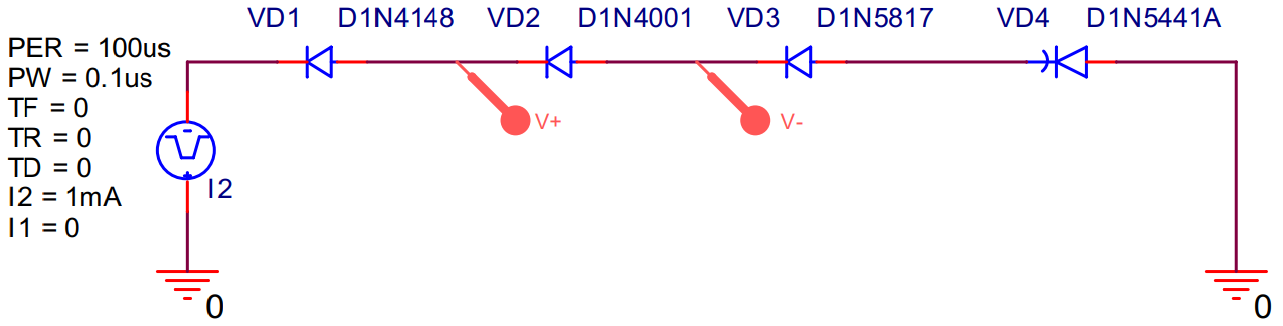
\includegraphics[width = 0.8 \textwidth]{scheme_1}
	\caption{Схемы моделирования вольт-амперных характеристик МОП транзисторов}
	\label{scheme_1}
\end{figure}

\begin{figure}[H]
	\centering
	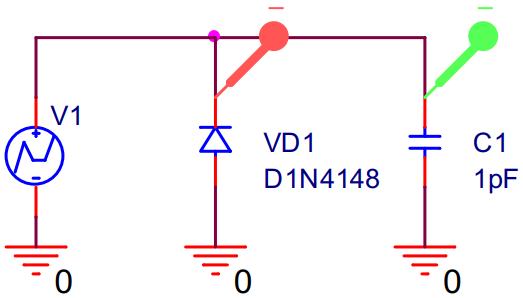
\includegraphics[width = 0.85 \textwidth]{scheme_2}
	\caption{Схемы моделирования емкости затворов МОП транзисторов}
	\label{scheme_2}
\end{figure}

\begin{figure}[H]
	\centering
	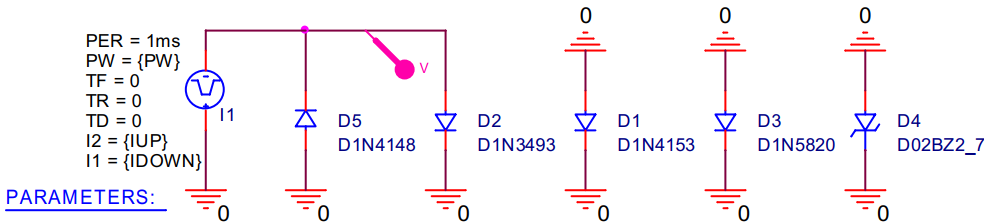
\includegraphics[width = 0.85 \textwidth]{scheme_3}
	\caption{Схемы моделирования переходных процессов МОП транзисторов}
	\label{scheme_3}
\end{figure}


\newpage




\section*{Выполнение}

\textbf{{\normalsize 1.n:}}
Составим схему (рис. \ref{scheme_1}) для n-канального МОП транзистора. Получим зависимость ID(M1) от напряжения V1 для трех значений температуры: $ \text{-}40\Cd, 27\Cd, 85\Cd $. По полученной зависимости определим U$_0$(M1) $ \approx 3.96 = \text{U}_0$.
\begin{figure}[H]
	\centering
	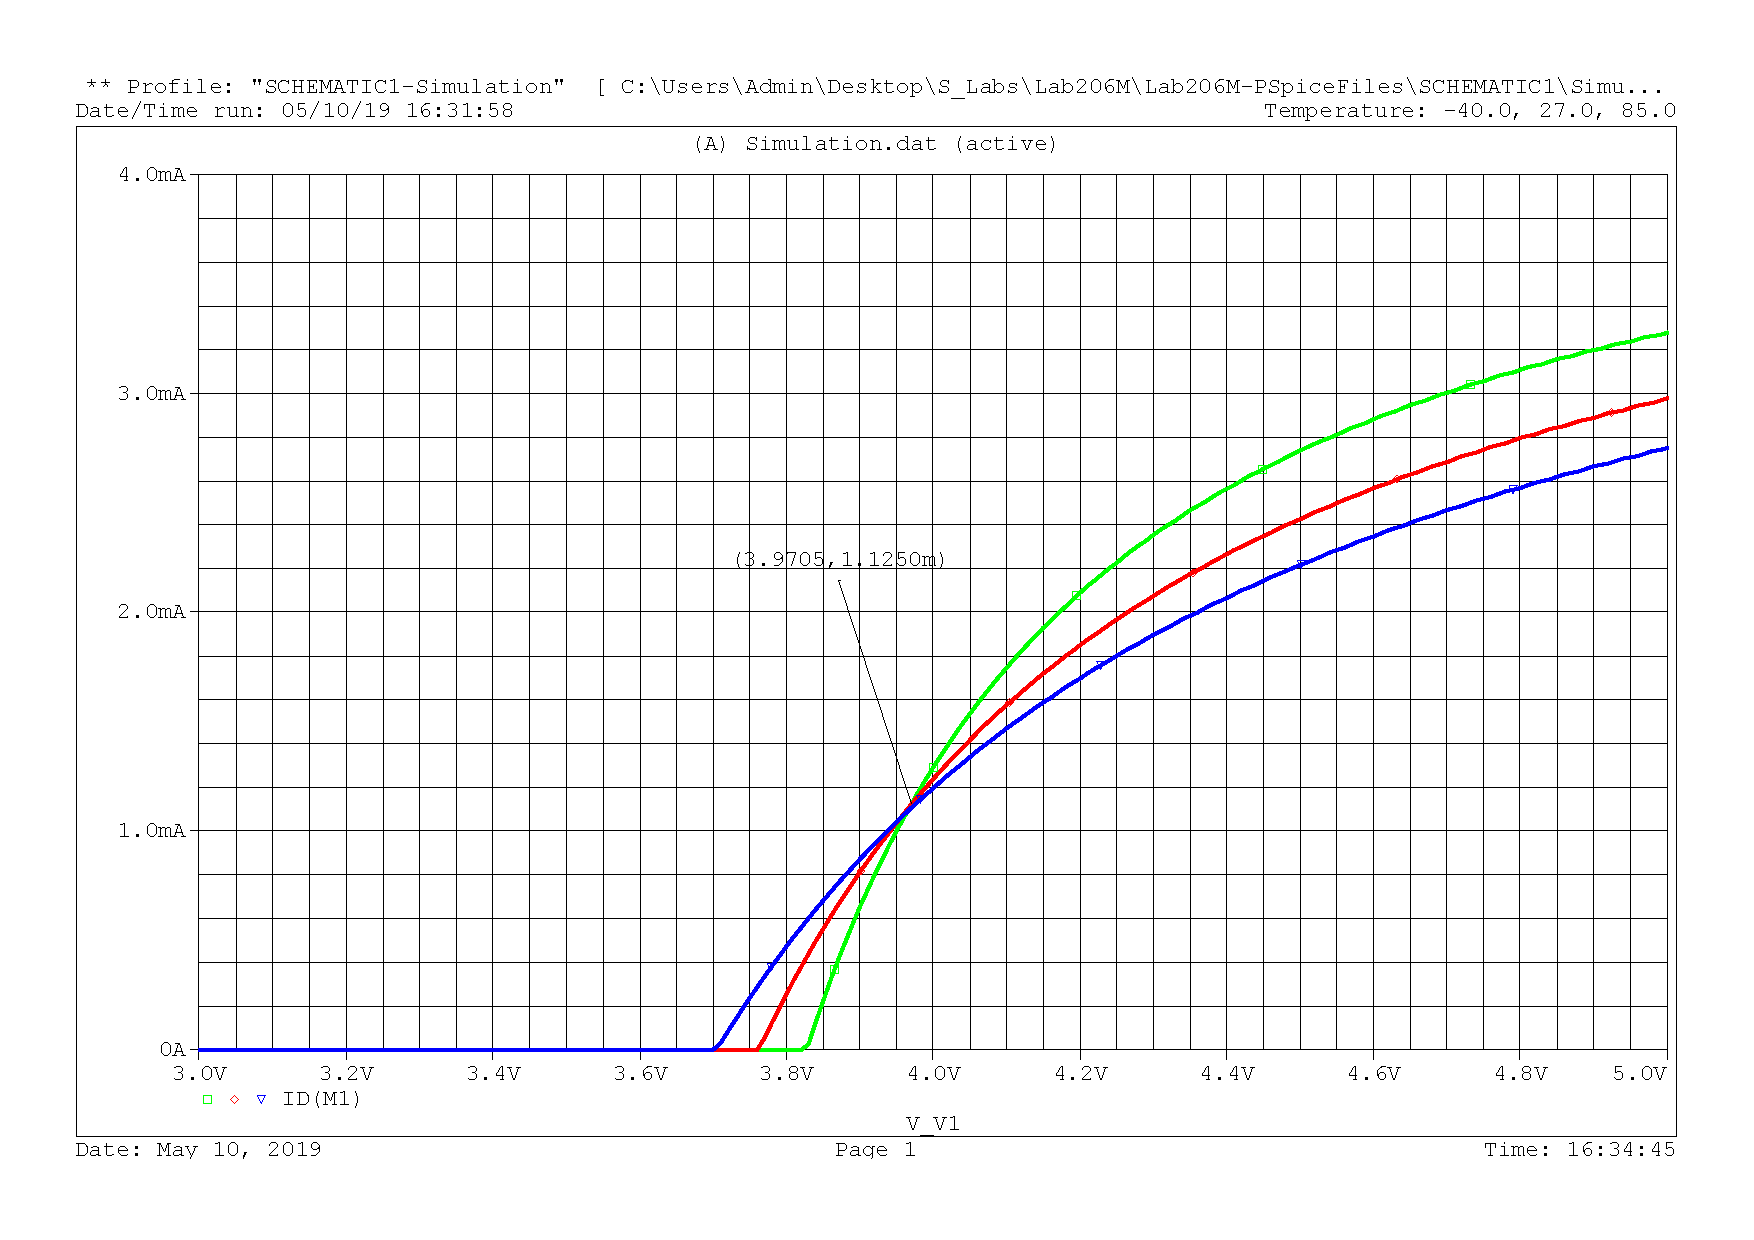
\includegraphics[width = 0.9 \textwidth]{1}
\end{figure}

\textbf{{\normalsize 1.p:}}
Составим схему (рис. \ref{scheme_1}) для p-канального МОП транзистора. Получим зависимость ID(M2) от напряжения V3 для трех значений температуры: $ \text{-}40\Cd, 27\Cd, 85\Cd $. По полученной зависимости определим U$_0$(M2) $ \approx \text{-}3.96 = \text{-U}_0$.
\begin{figure}[H]
	\centering
	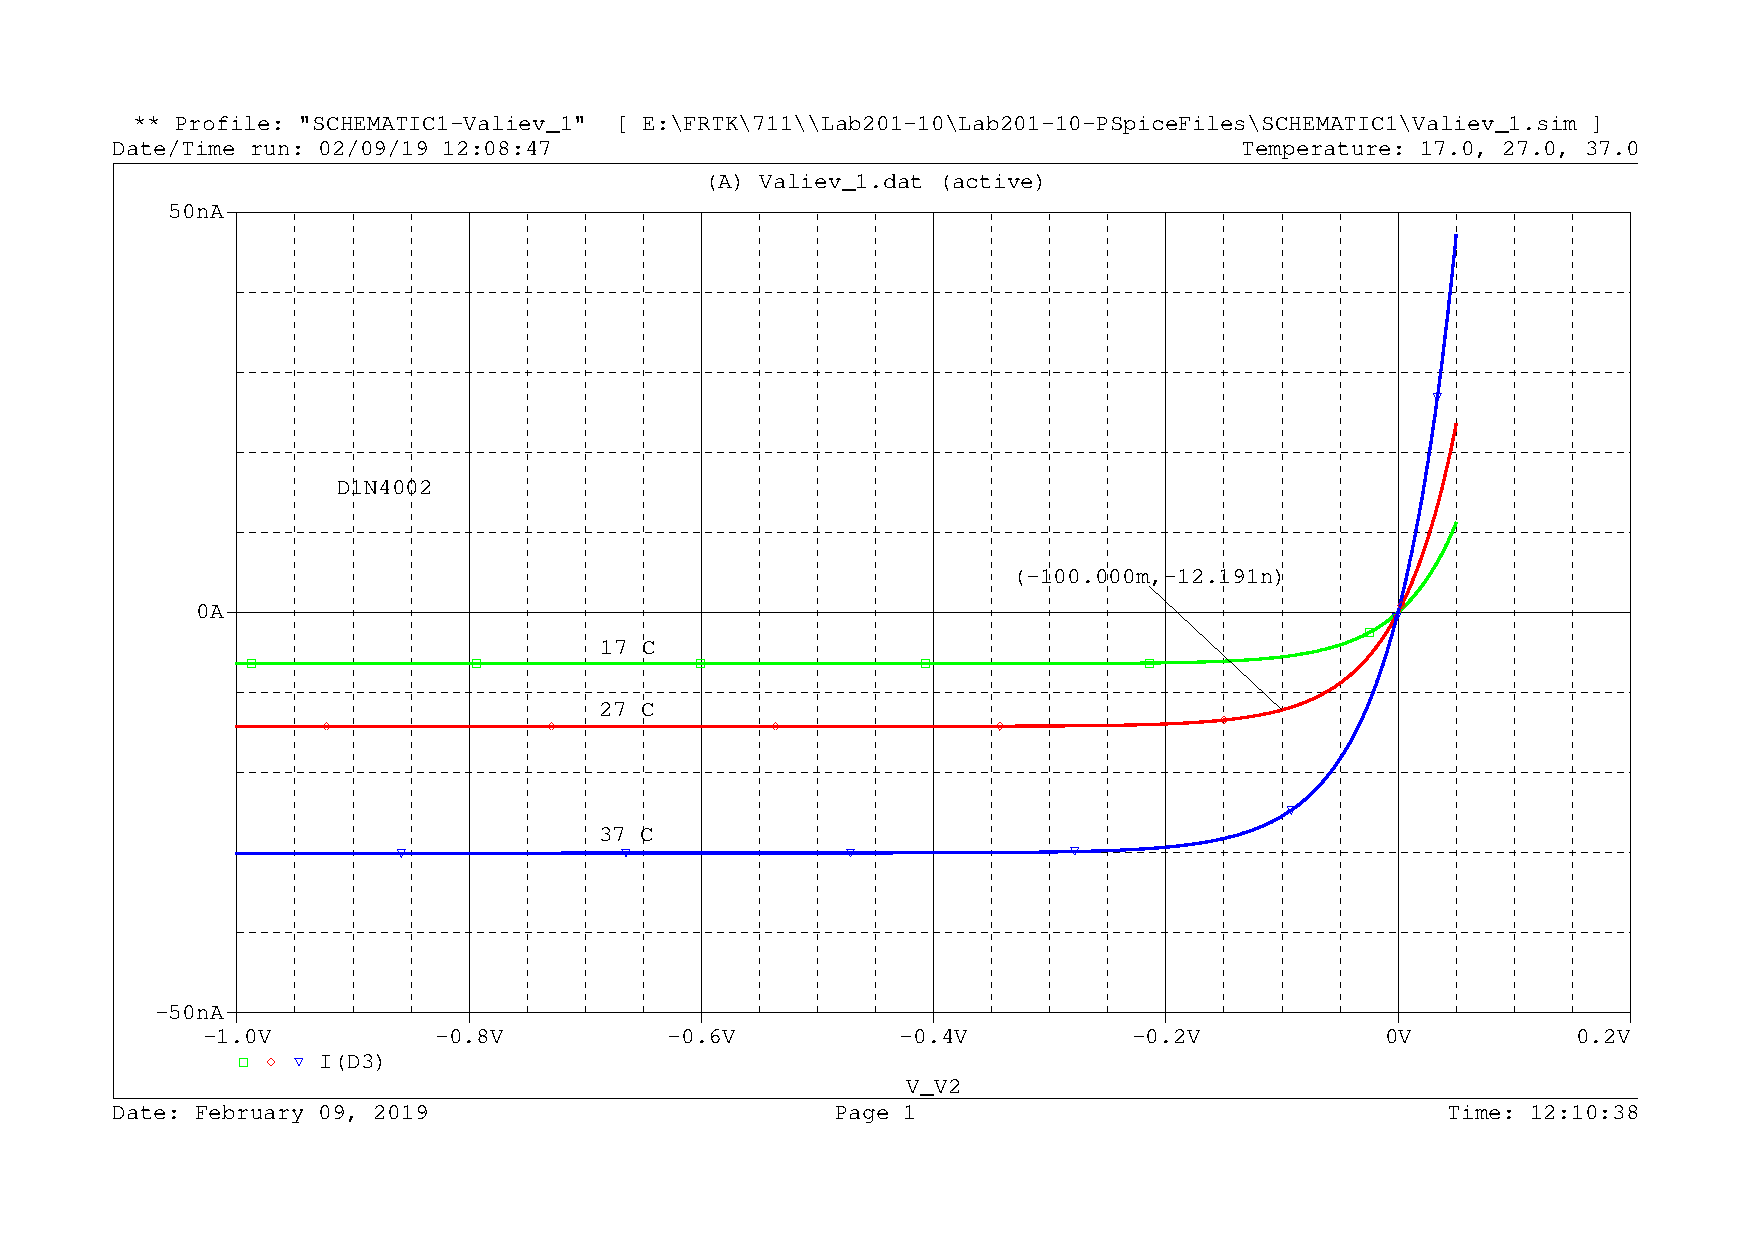
\includegraphics[width = 0.9 \textwidth]{2}
\end{figure}

\newpage





\textbf{{\normalsize 2.n:}}
Установим напряжение V2 = 5V. Получим зависимость тока стока ID(M1) от напряжения на источнике V1 в диапазоне от U$_0$(M1) до 5V для трех значений температуры: $ \text{-}40\Cd, 27\Cd, 85\Cd $.
\begin{figure}[H]
	\centering
	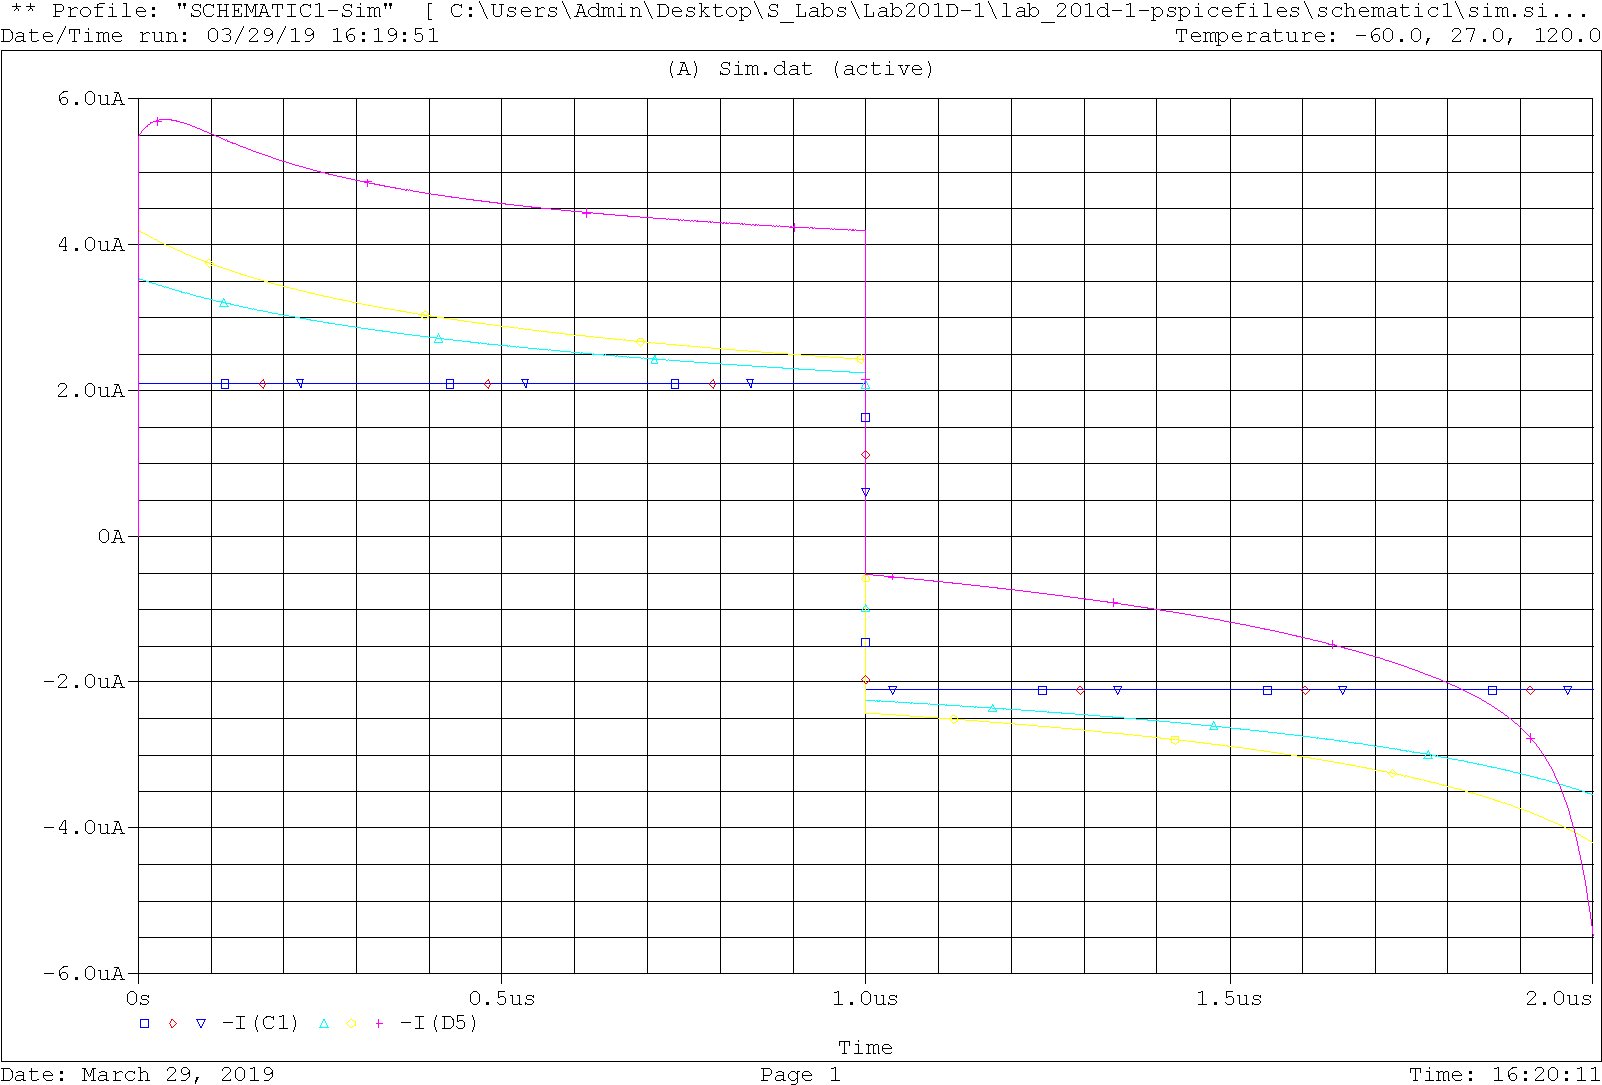
\includegraphics[width = 0.9 \textwidth]{3}
\end{figure}

\textbf{{\normalsize 2.p:}}
Установим напряжение V4 = -5V. Получим зависимость тока стока ID(M2) от напряжения на источнике V3 в диапазоне от -5V до U$_0$(M2) для трех значений температуры: $ \text{-}40\Cd, 27\Cd, 85\Cd $.
\begin{figure}[H]
	\centering
	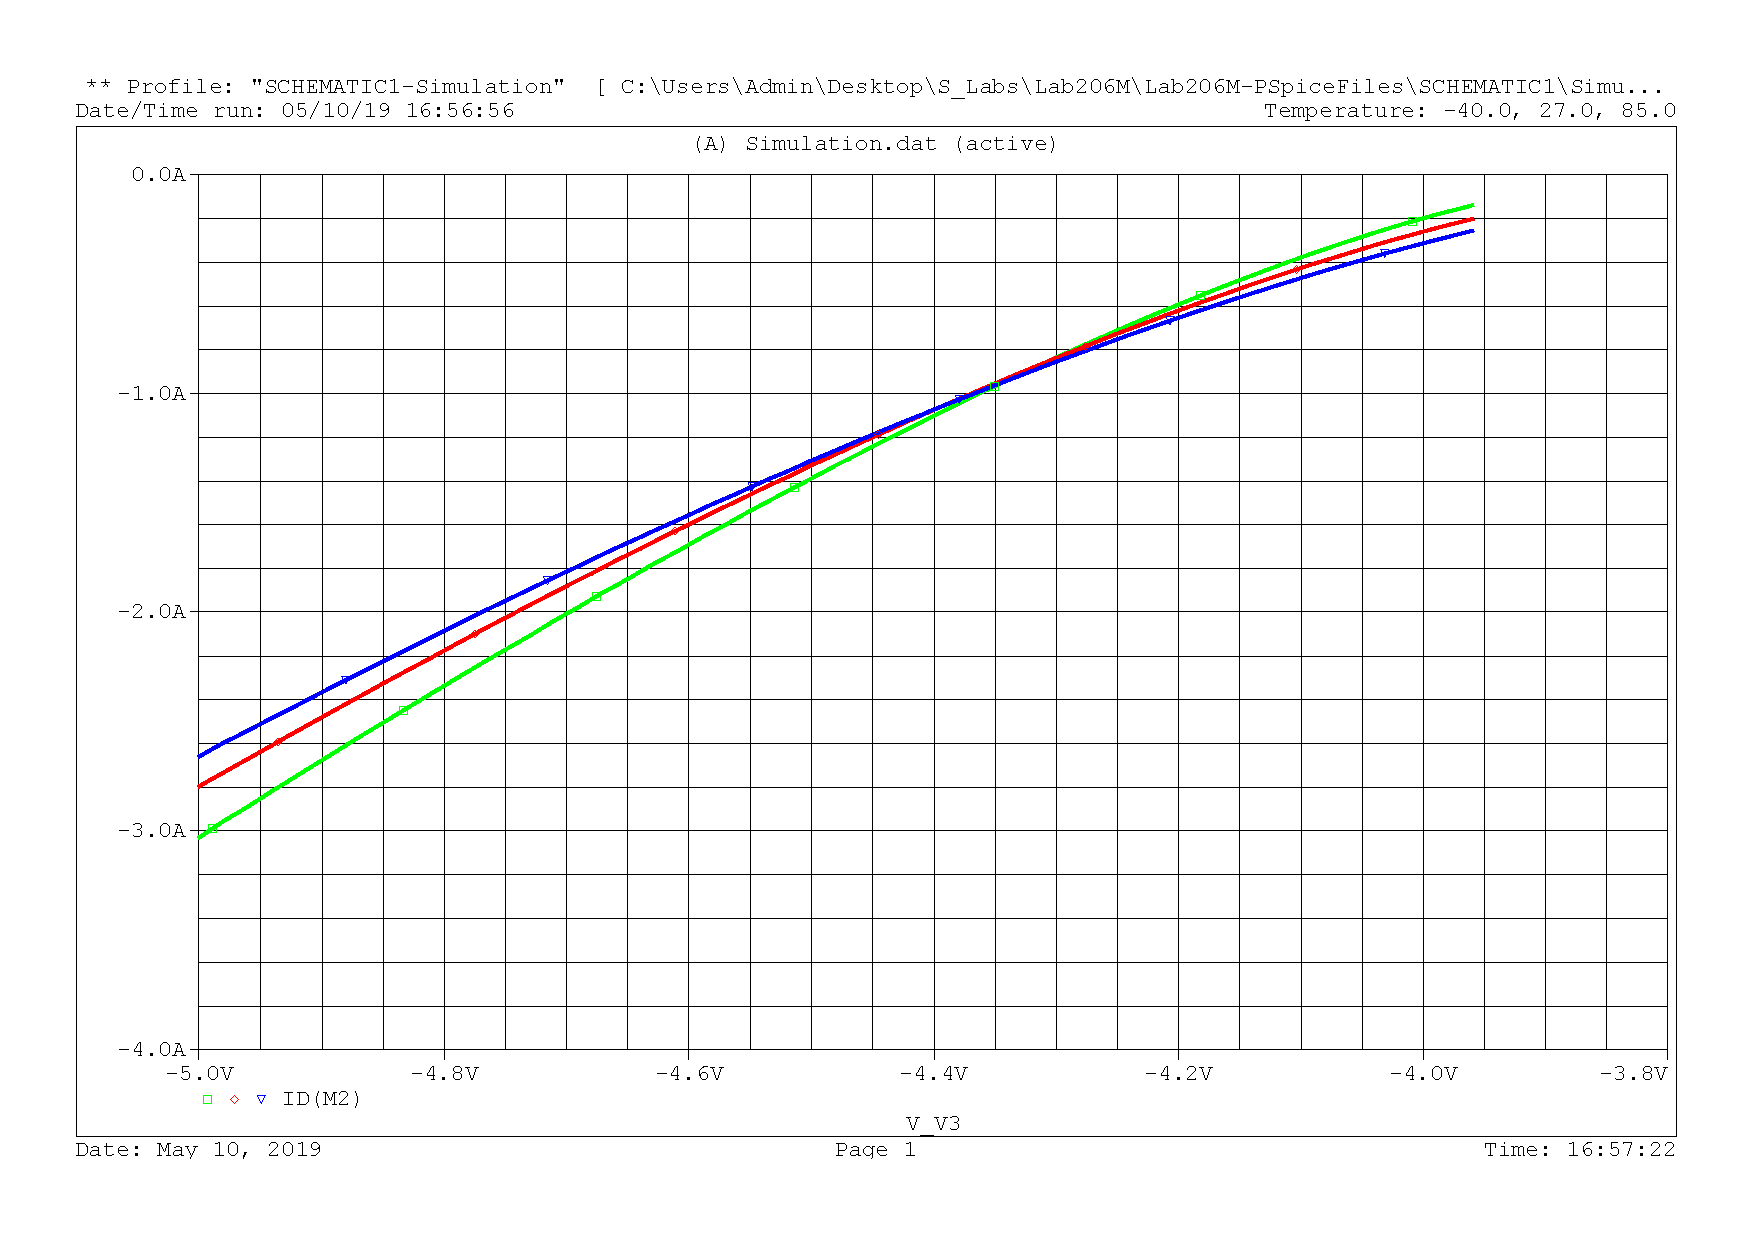
\includegraphics[width = 0.9 \textwidth]{4}
\end{figure}

\newpage





\textbf{{\normalsize 3.n.1:}}
Получим зависимость тока стока ID(M1) от напряжения источника V2 для некоторых значений напряжения V1 от U$_0$ до 5V.
\begin{figure}[H]
	\centering
	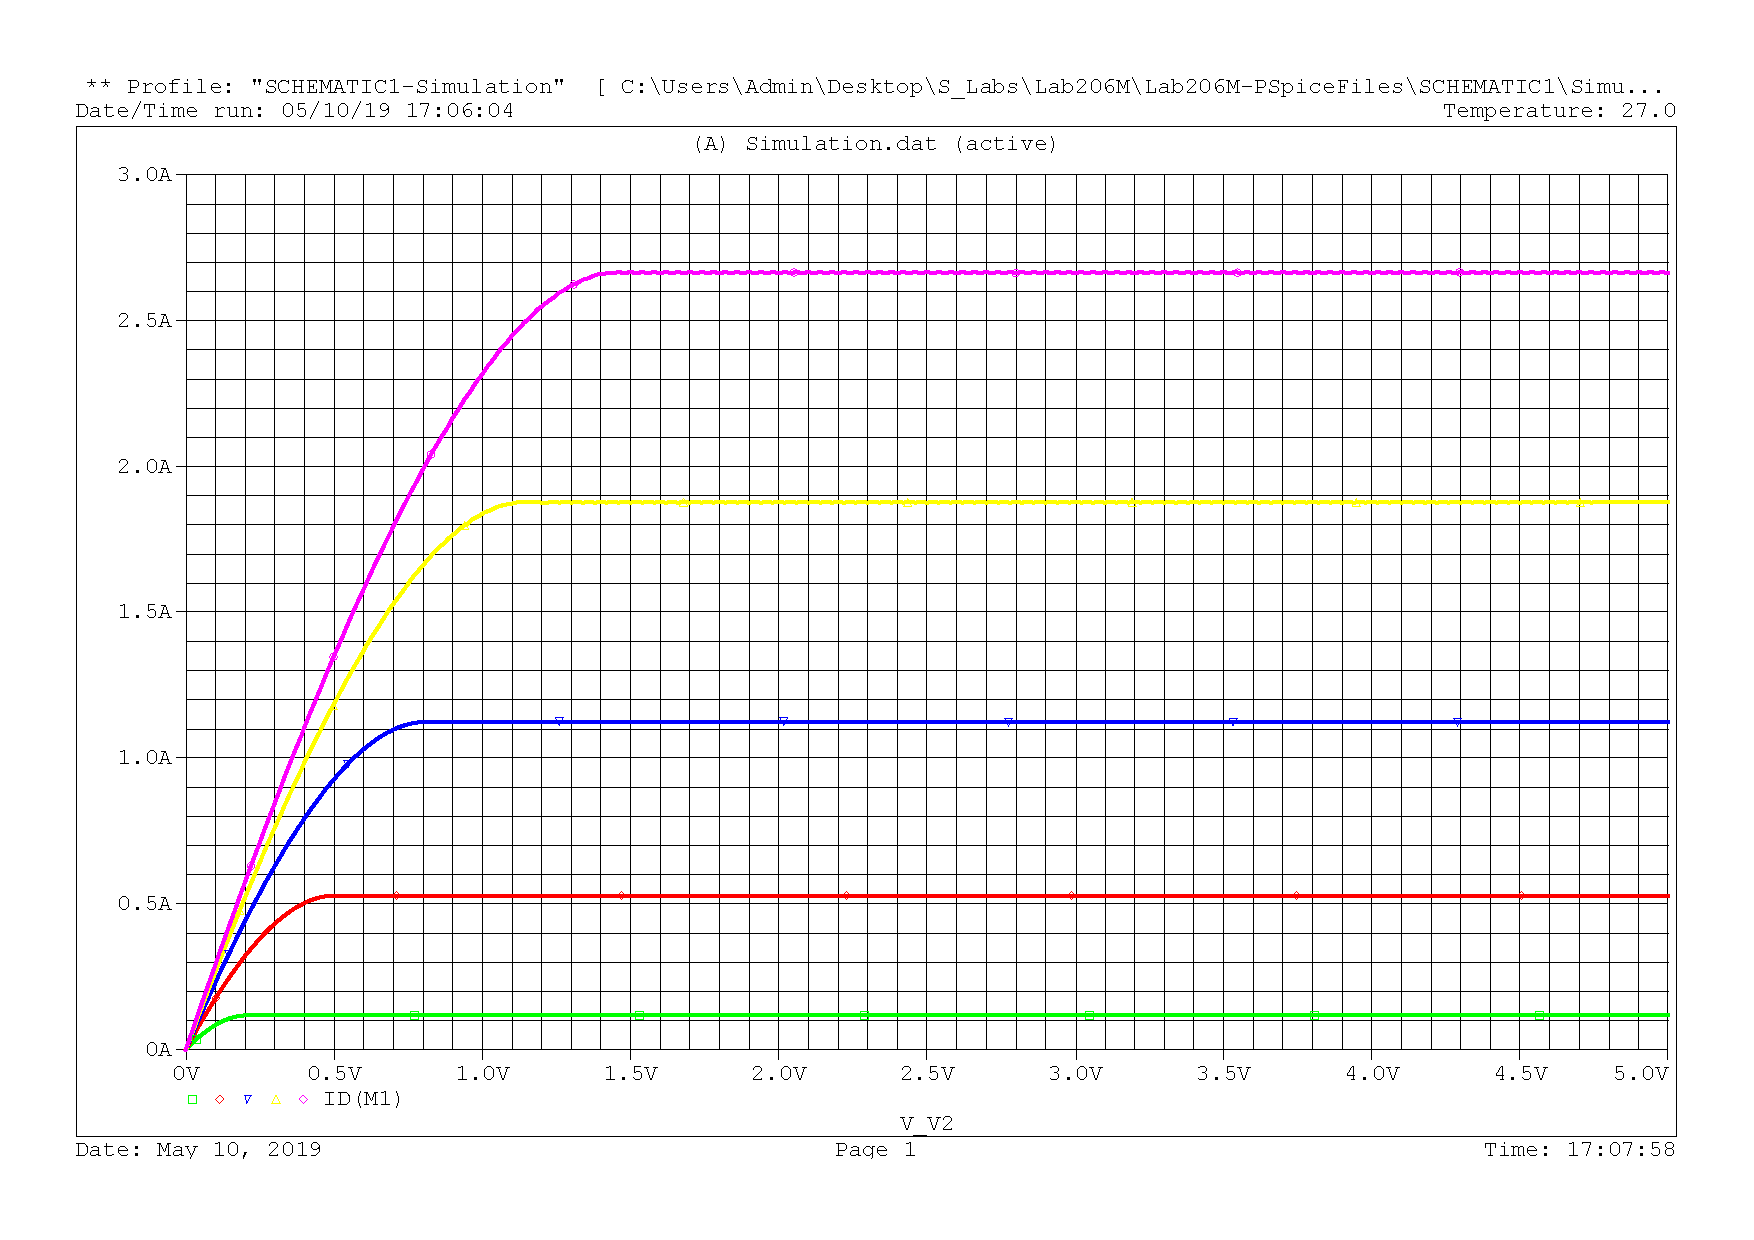
\includegraphics[width = 0.9 \textwidth]{5}
\end{figure}

\textbf{{\normalsize 3.n.2:}}
Повторим предыдущий пункт для трех значений напряжения V1 на затворе: 4.9V, 5V, 5.1V. Определим по полученным результатам g$_{\text{m}}$(M1), g$_{\text{i}}$(M1), U$_{\text{A}}$(M1), M(M1) = g$_{\text{m}}$(M1)/g$_{\text{i}}$(M1).
\begin{figure}[H]
	\centering
	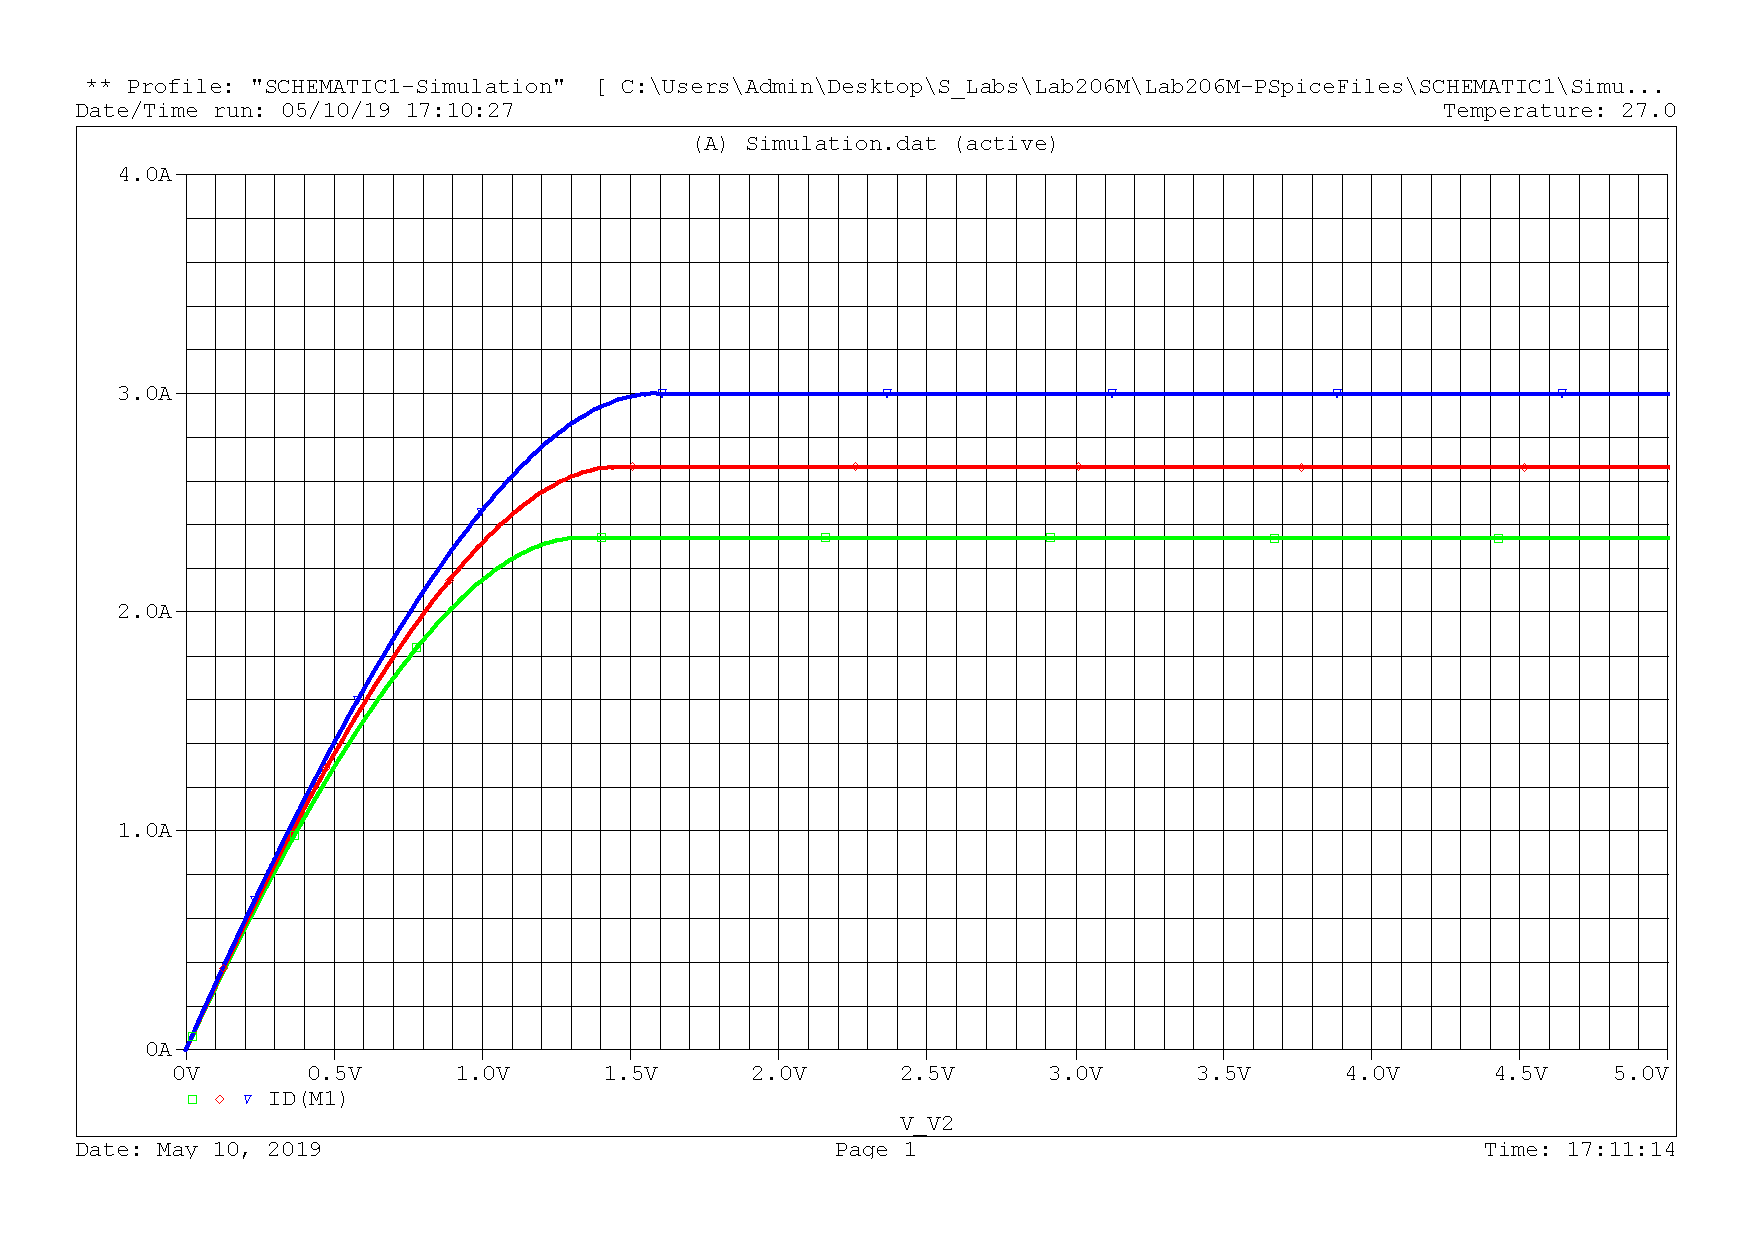
\includegraphics[width = 0.9 \textwidth]{6}
	\caption{g$_{\text{m}}\text{(M1)} \approx 4.3$; g$_{\text{i}}\text{(M1)} \approx 3.1$; U$_{\text{A}}\text{(M1)} \approx 1.4$; M(M1) $\approx$ 1.39}
\end{figure}

\newpage

\textbf{{\normalsize 3.n.3:}}
Установим напряжение источника V1 = 5V получим зависимость тока стока ID(M1) от напряжения на источнике V2 для трех значений температуры: $ \text{-}40\Cd, 27\Cd, 85\Cd $.
\begin{figure}[H]
	\centering
	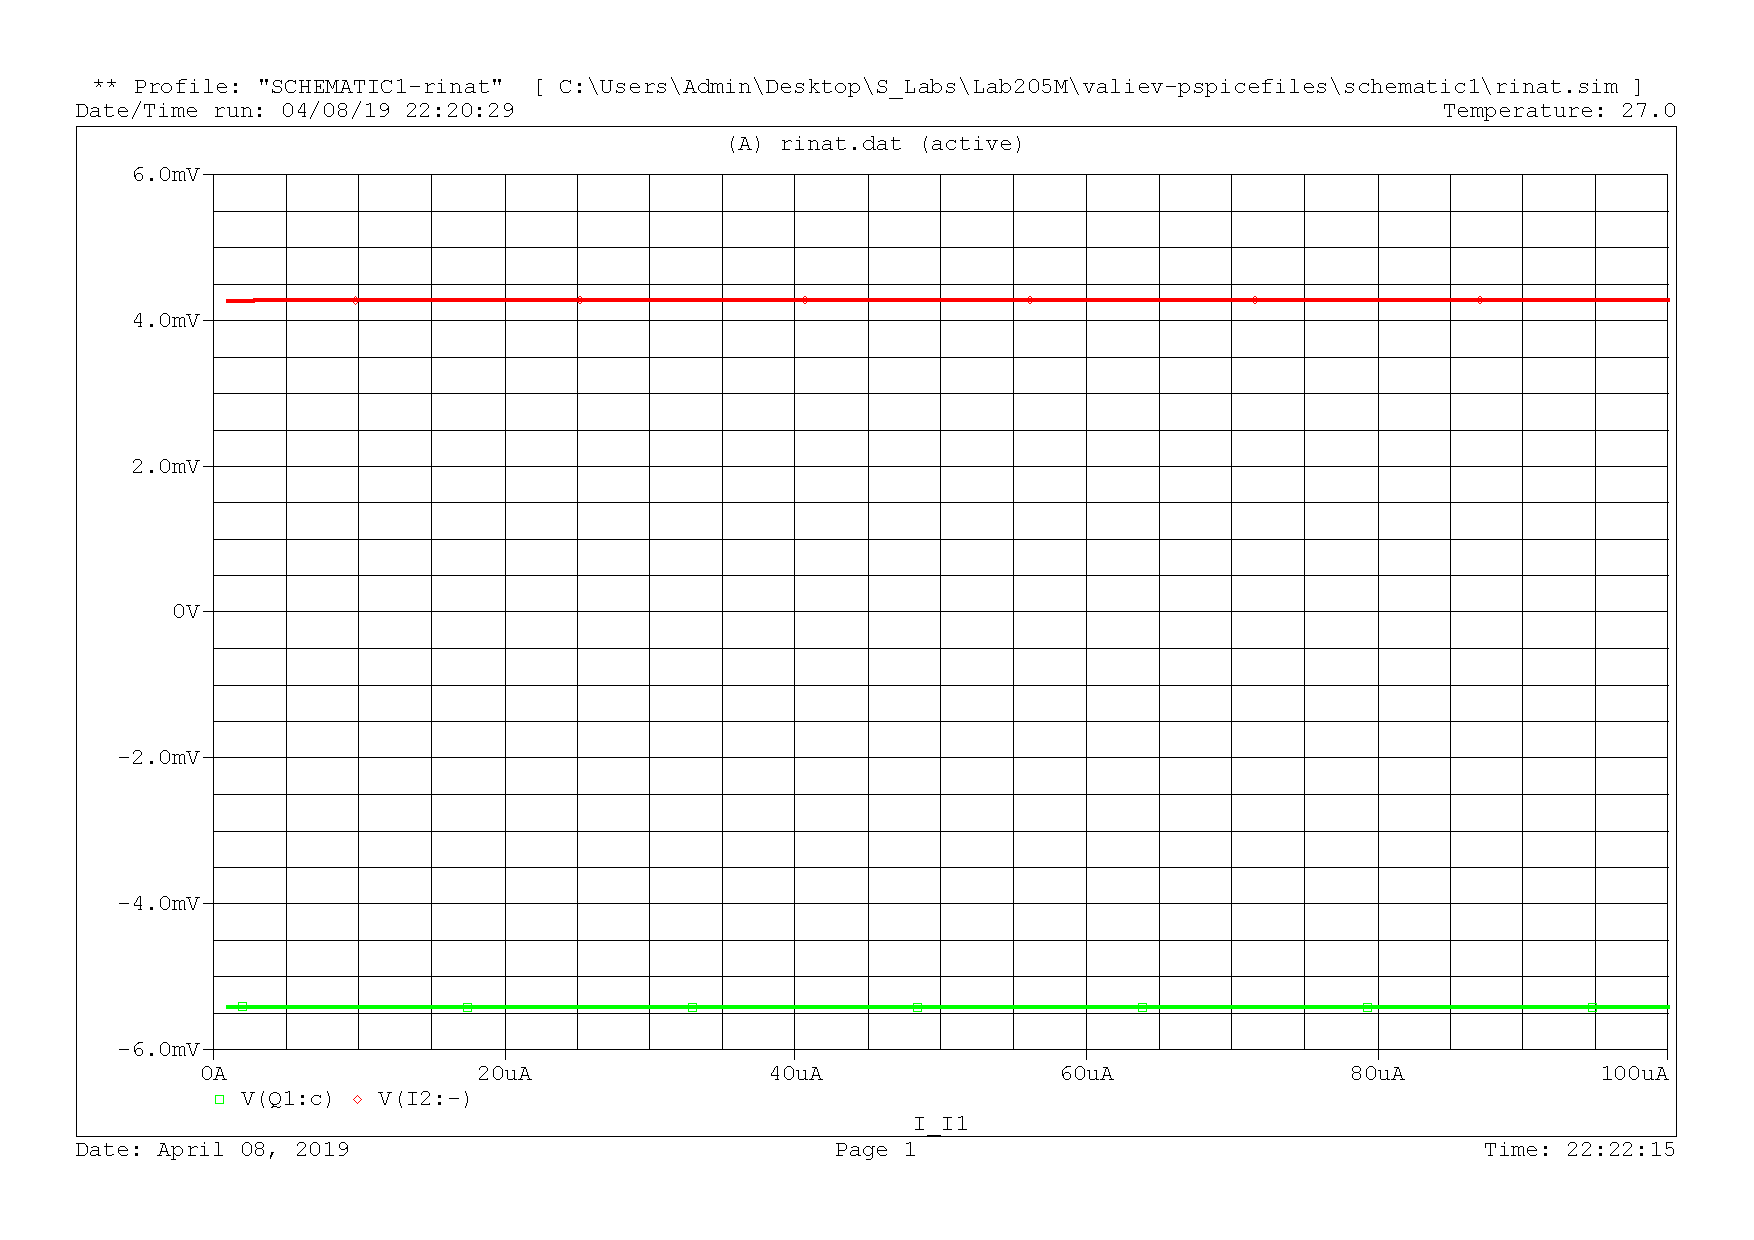
\includegraphics[width = 0.9 \textwidth]{7}
\end{figure}

\textbf{{\normalsize 3.n.4:}}
При V1 = V2 = 5V получим зависимость тока стока ID(M1) от температуры.
\begin{figure}[H]
\centering
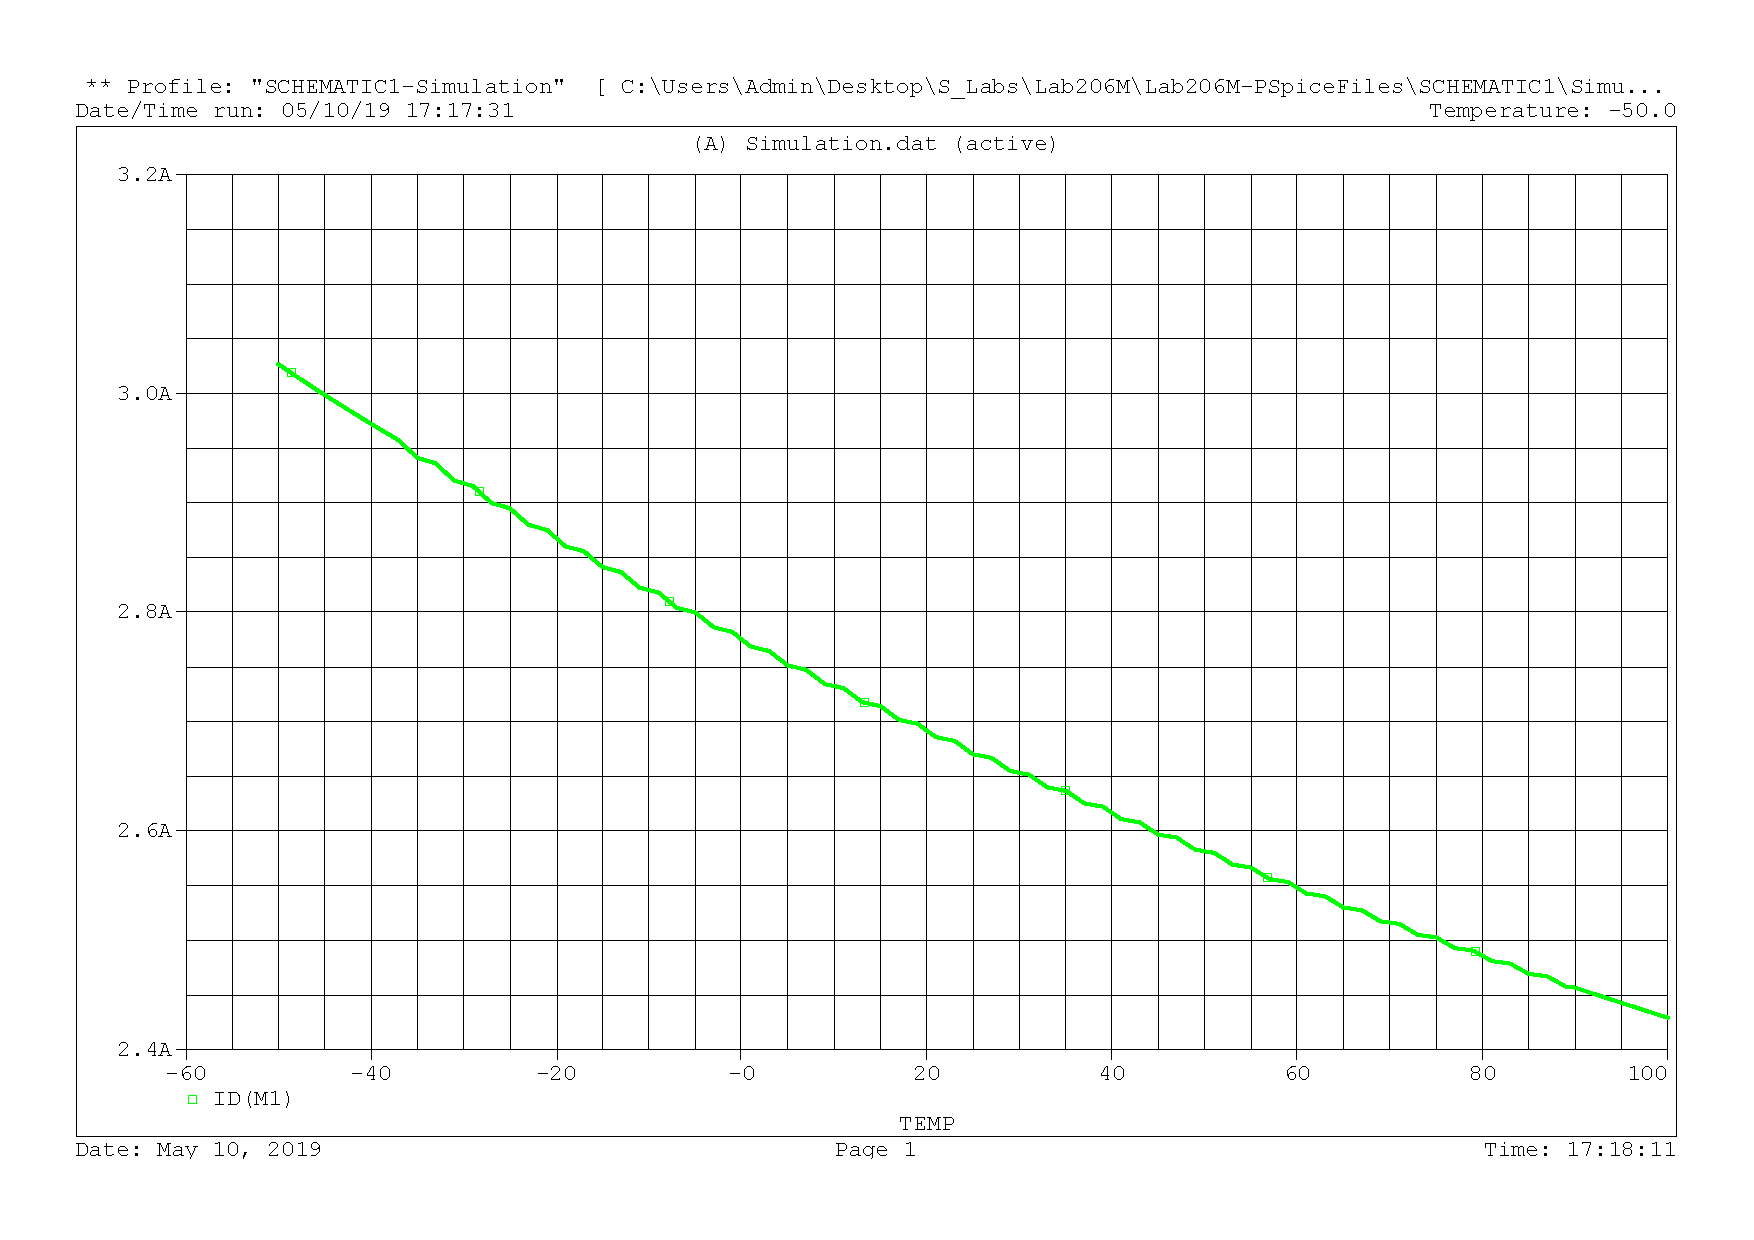
\includegraphics[width = 0.9 \textwidth]{8}
\end{figure}

\newpage





\textbf{{\normalsize 3.p.1:}}
Получим зависимость тока стока ID(M2) от напряжения источника V4 для некоторых значений напряжения V3 от -5V до -U$_0$.
\begin{figure}[H]
	\centering
	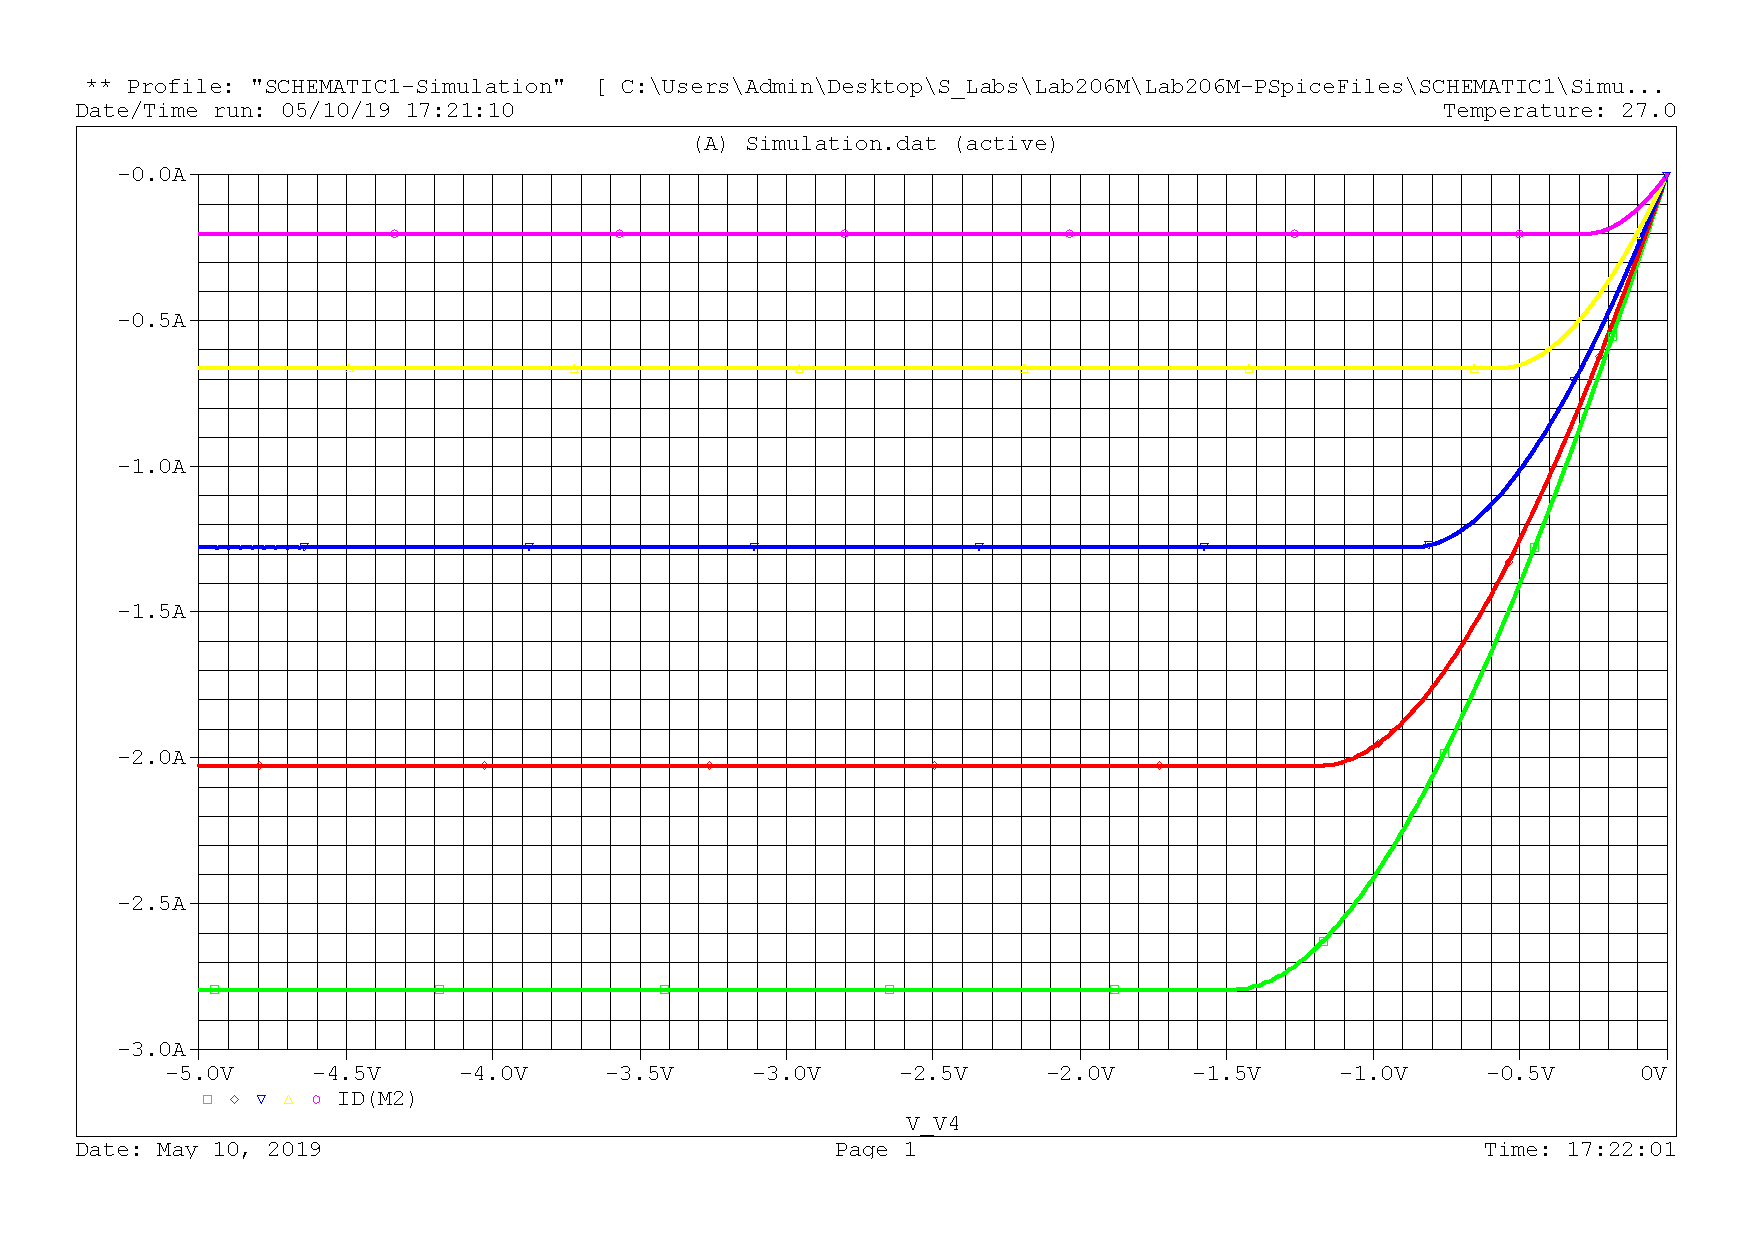
\includegraphics[width = 0.9 \textwidth]{9}
\end{figure}

\textbf{{\normalsize 3.p.2:}}
Повторим предыдущий пункт для трех значений напряжения V3 на затворе: -5.1V, -5V, -4.9V. Определим по полученным результатам g$_{\text{m}}$(M2), g$_{\text{i}}$(M2), U$_{\text{A}}$(M2), M(M2) = g$_{\text{m}}$(M2)/g$_{\text{i}}$(M2).
\begin{figure}[H]
	\centering
	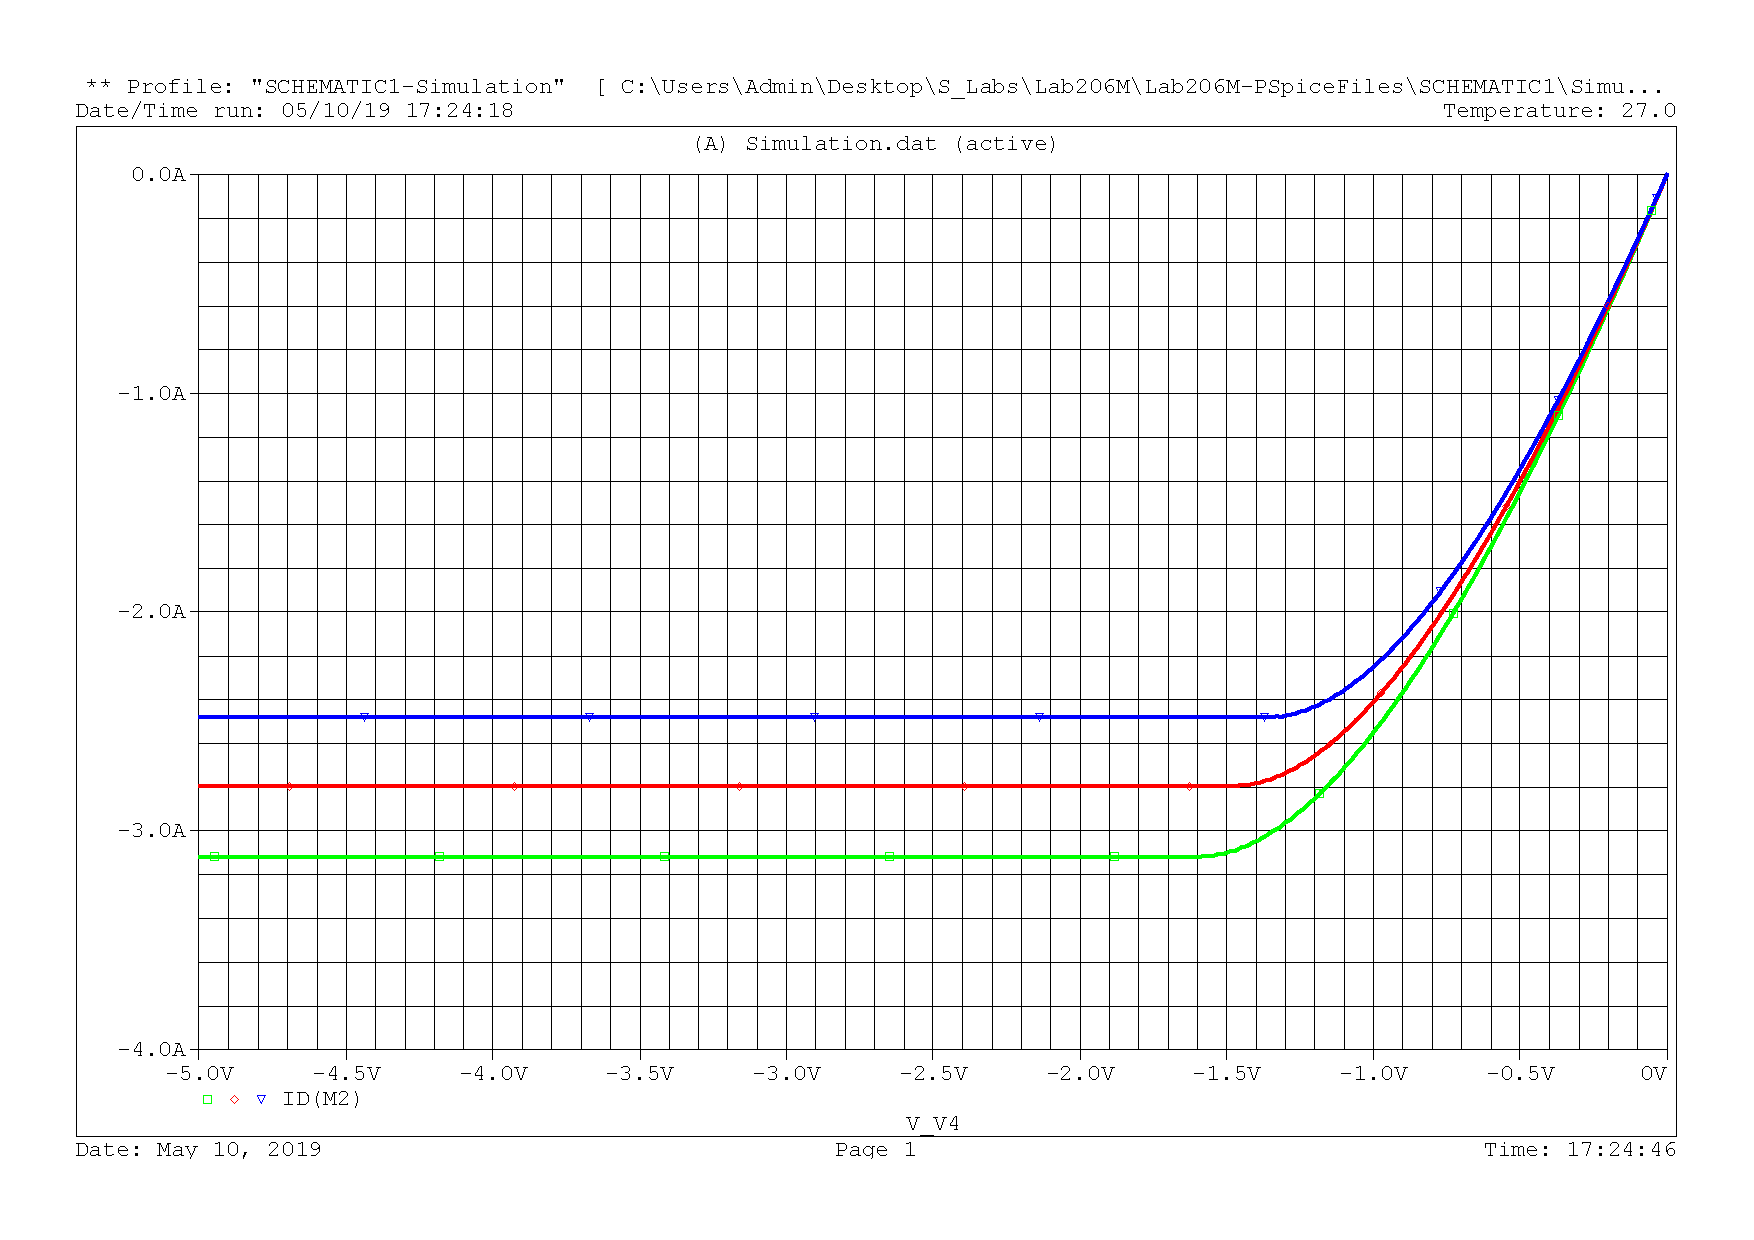
\includegraphics[width = 0.9 \textwidth]{10}
	\caption{g$_{\text{m}}\text{(M2)} \approx 4.8$; g$_{\text{i}}\text{(M2)} \approx 3.4$; U$_{\text{A}}\text{(M2)} \approx -1.4$; M(M2) $\approx$ 1.41}
\end{figure}

\newpage

\textbf{{\normalsize 3.p.3:}}
Установим напряжение источника V3 = -5V получим зависимость тока стока ID(M2) от напряжения на источнике V4 для трех значений температуры: $ \text{-}40\Cd, 27\Cd, 85\Cd $.
\begin{figure}[H]
	\centering
	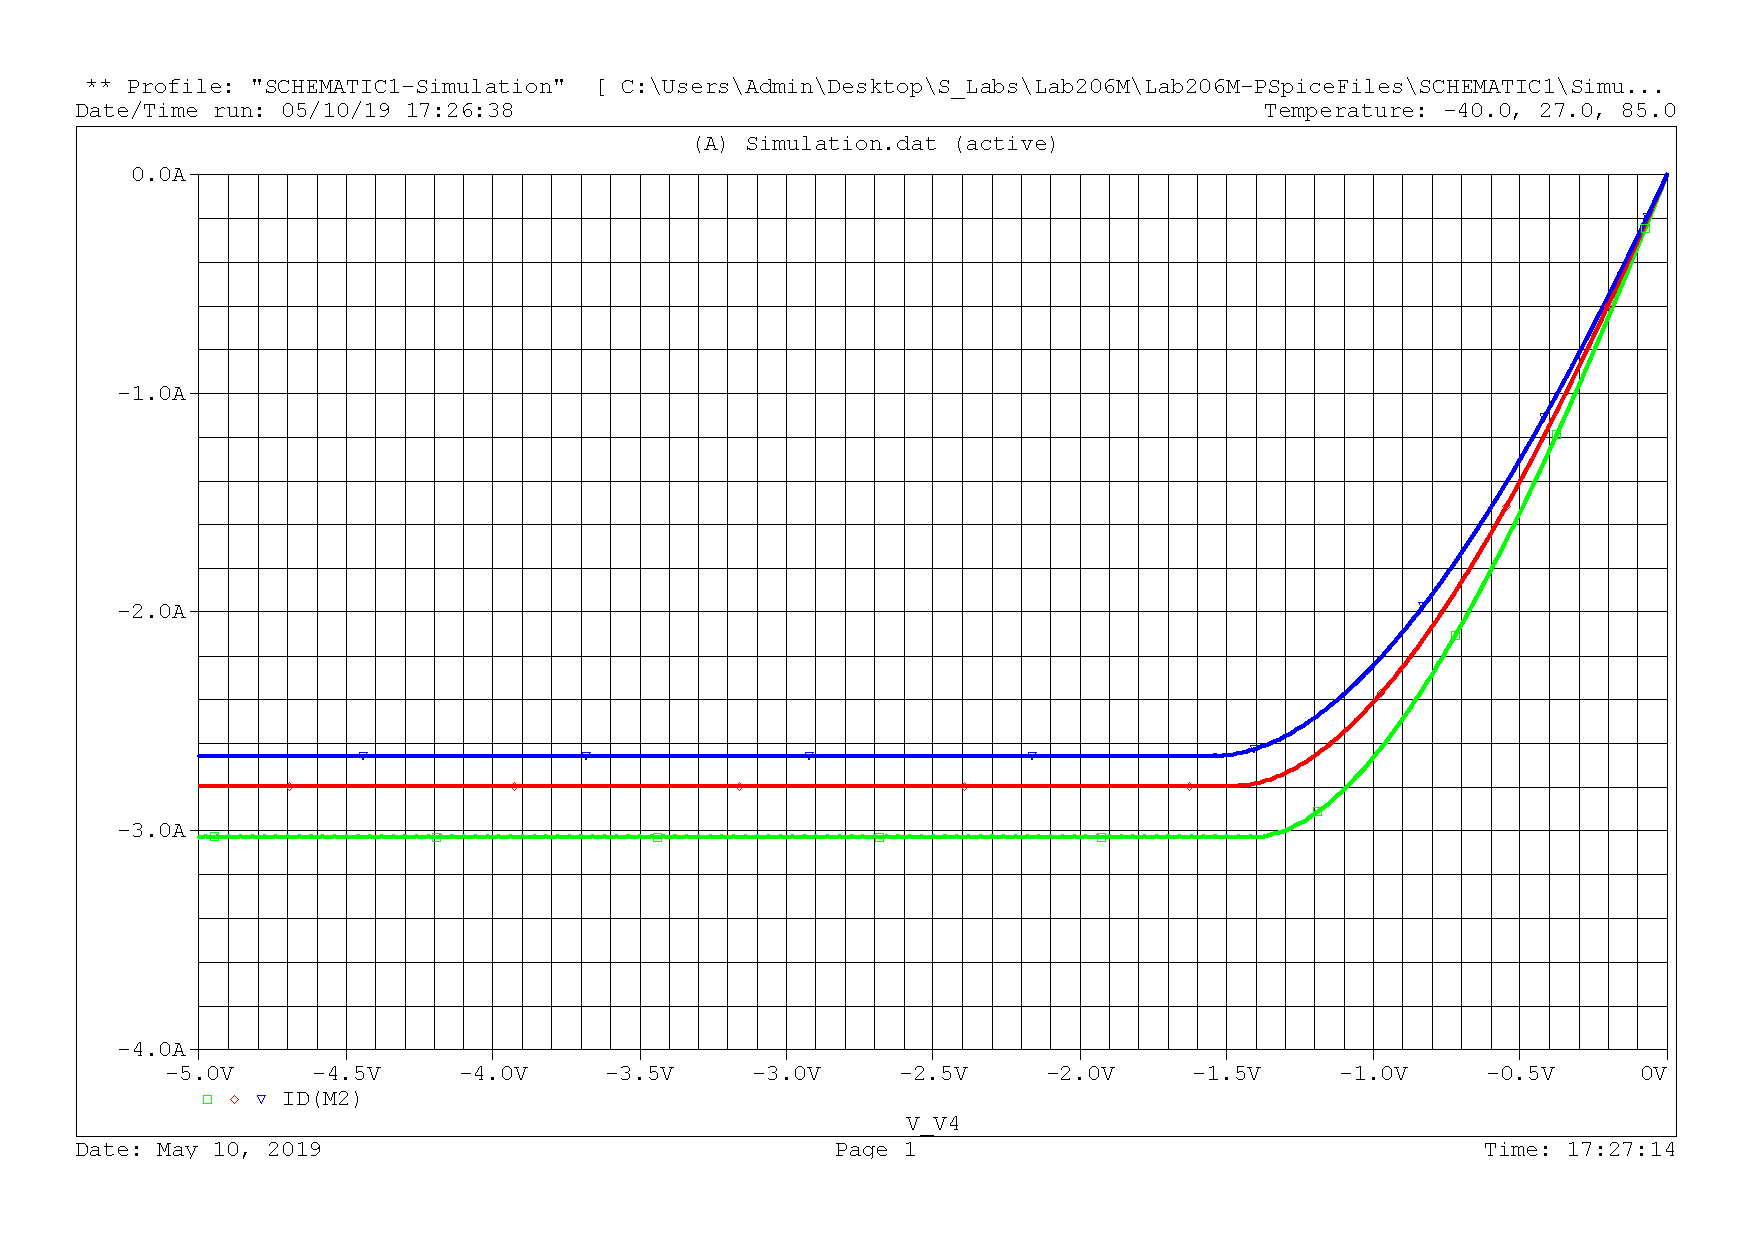
\includegraphics[width = 0.9 \textwidth]{11}
\end{figure}

\textbf{{\normalsize 3.p.4:}}
При V3 = V4 = -5V получим зависимость тока стока ID(M2) от температуры.
\begin{figure}[H]
	\centering
	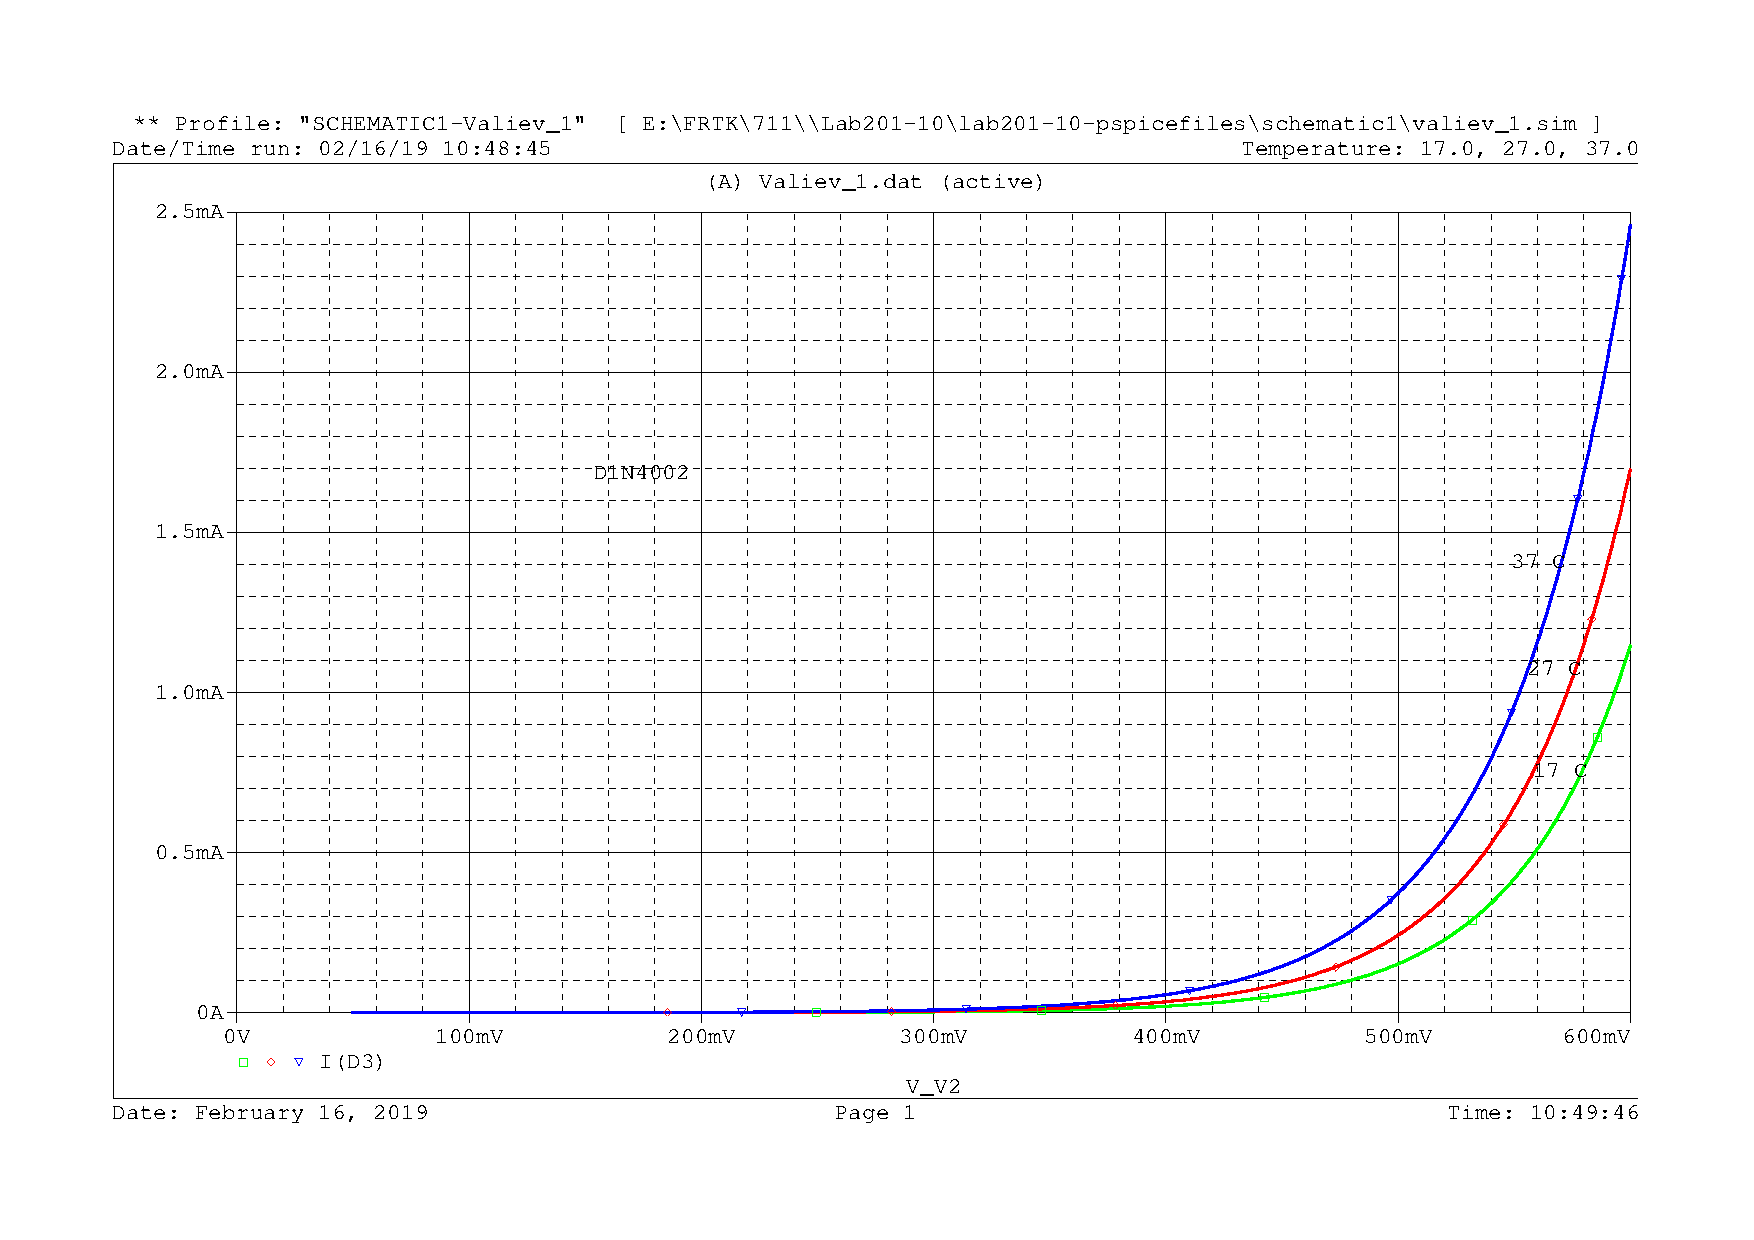
\includegraphics[width = 0.9 \textwidth]{12}
\end{figure}

\newpage





\textbf{{\normalsize 4.1:}}
Составим схему (рис. \ref{scheme_2}) моделирования емкости затворов МОП транзисторов. Получим временные диаграммы токов затворов IG(M1), IG(M2) для двух значений сопротивления резисторов нагрузки R1, R2: 0.1, 100.
\begin{figure}[H]
	\centering
	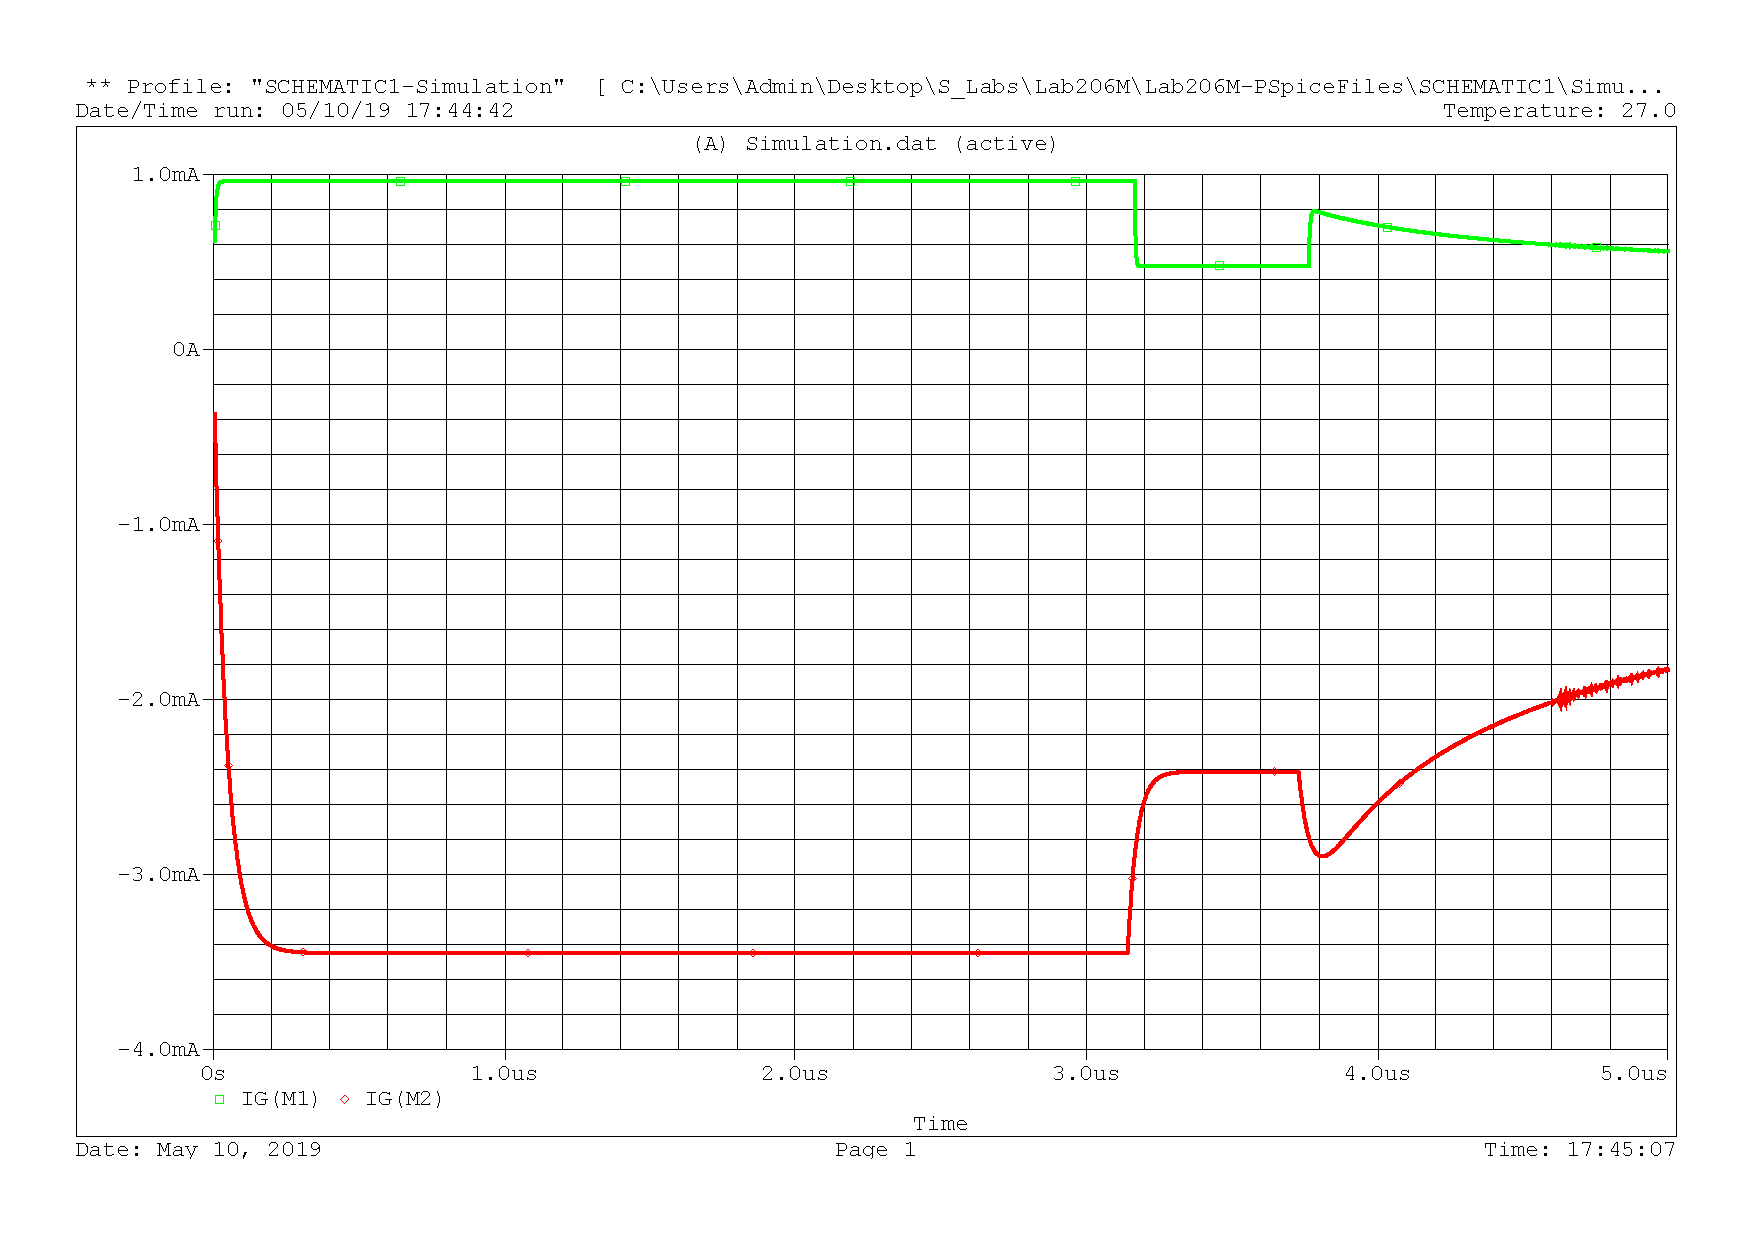
\includegraphics[width = 0.9 \textwidth]{13}
	\caption{R1 = R2 = 0.1}
\end{figure}

\begin{figure}[H]
	\centering
	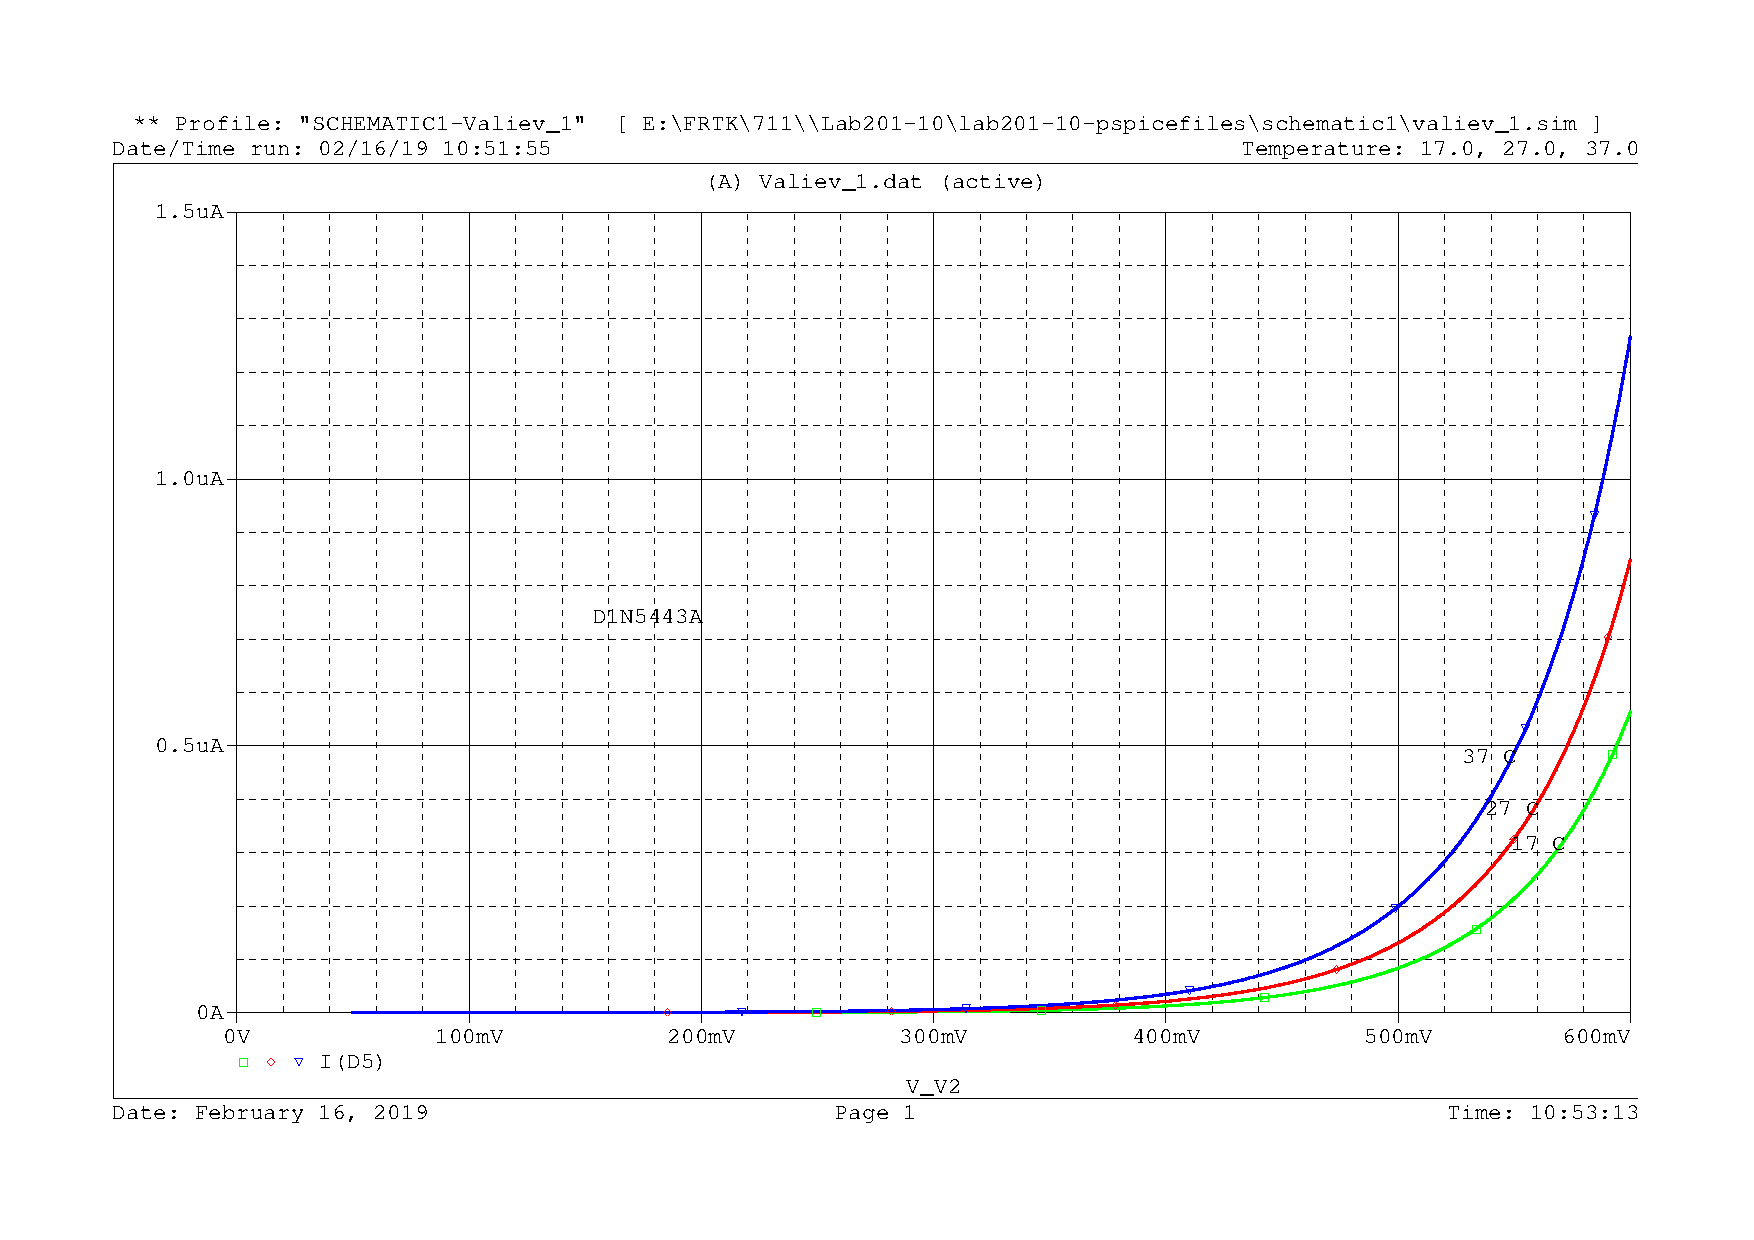
\includegraphics[width = 0.9 \textwidth]{14}
	\caption{R1 = R2 = 100}
\end{figure}

\textbf{{\normalsize 4.2:}}
При тех же значениях R1 и R2 получим временные диаграммы напряжений на стоках UG(M1), UG(M2).
\begin{figure}[H]
	\centering
	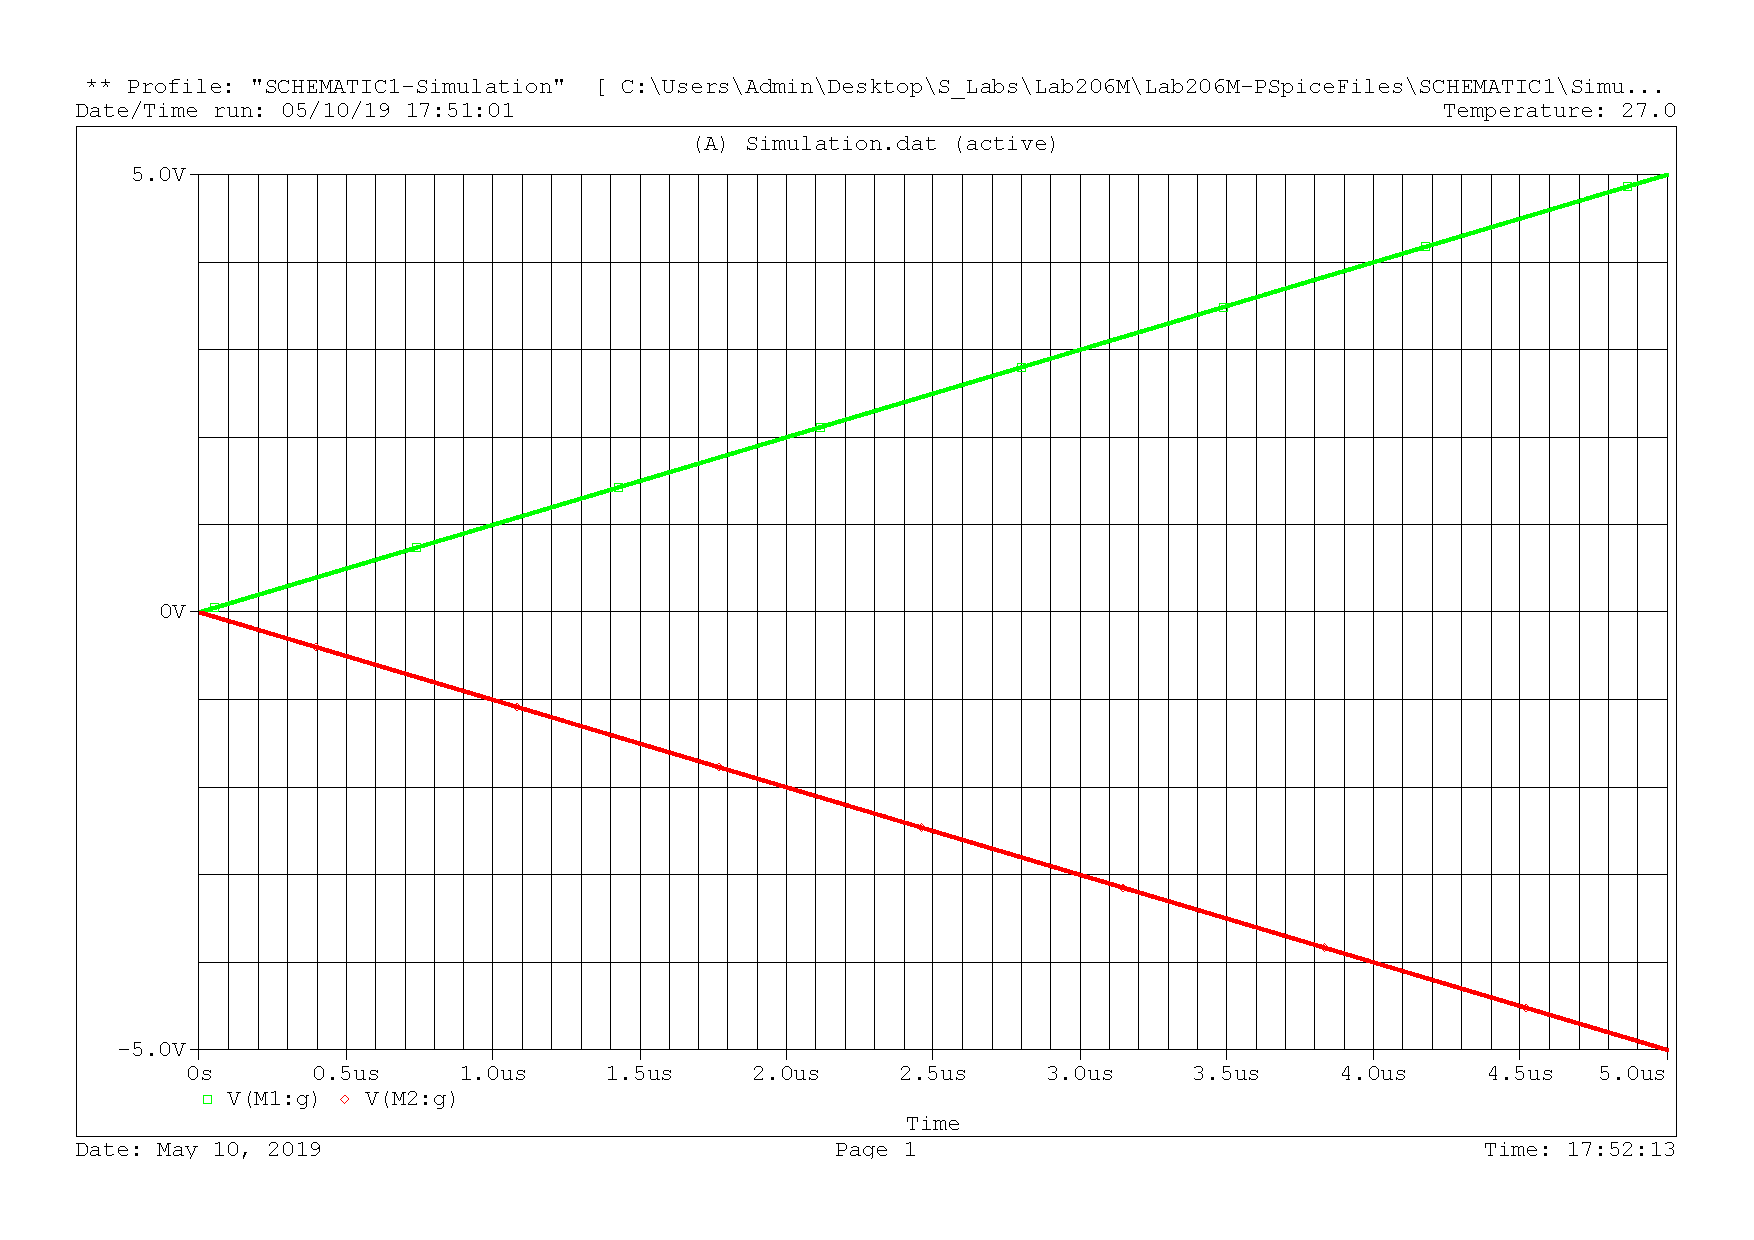
\includegraphics[width = 0.9 \textwidth]{15}
	\caption{R1 = R2 = 0.1}
\end{figure}

\begin{figure}[H]
	\centering
	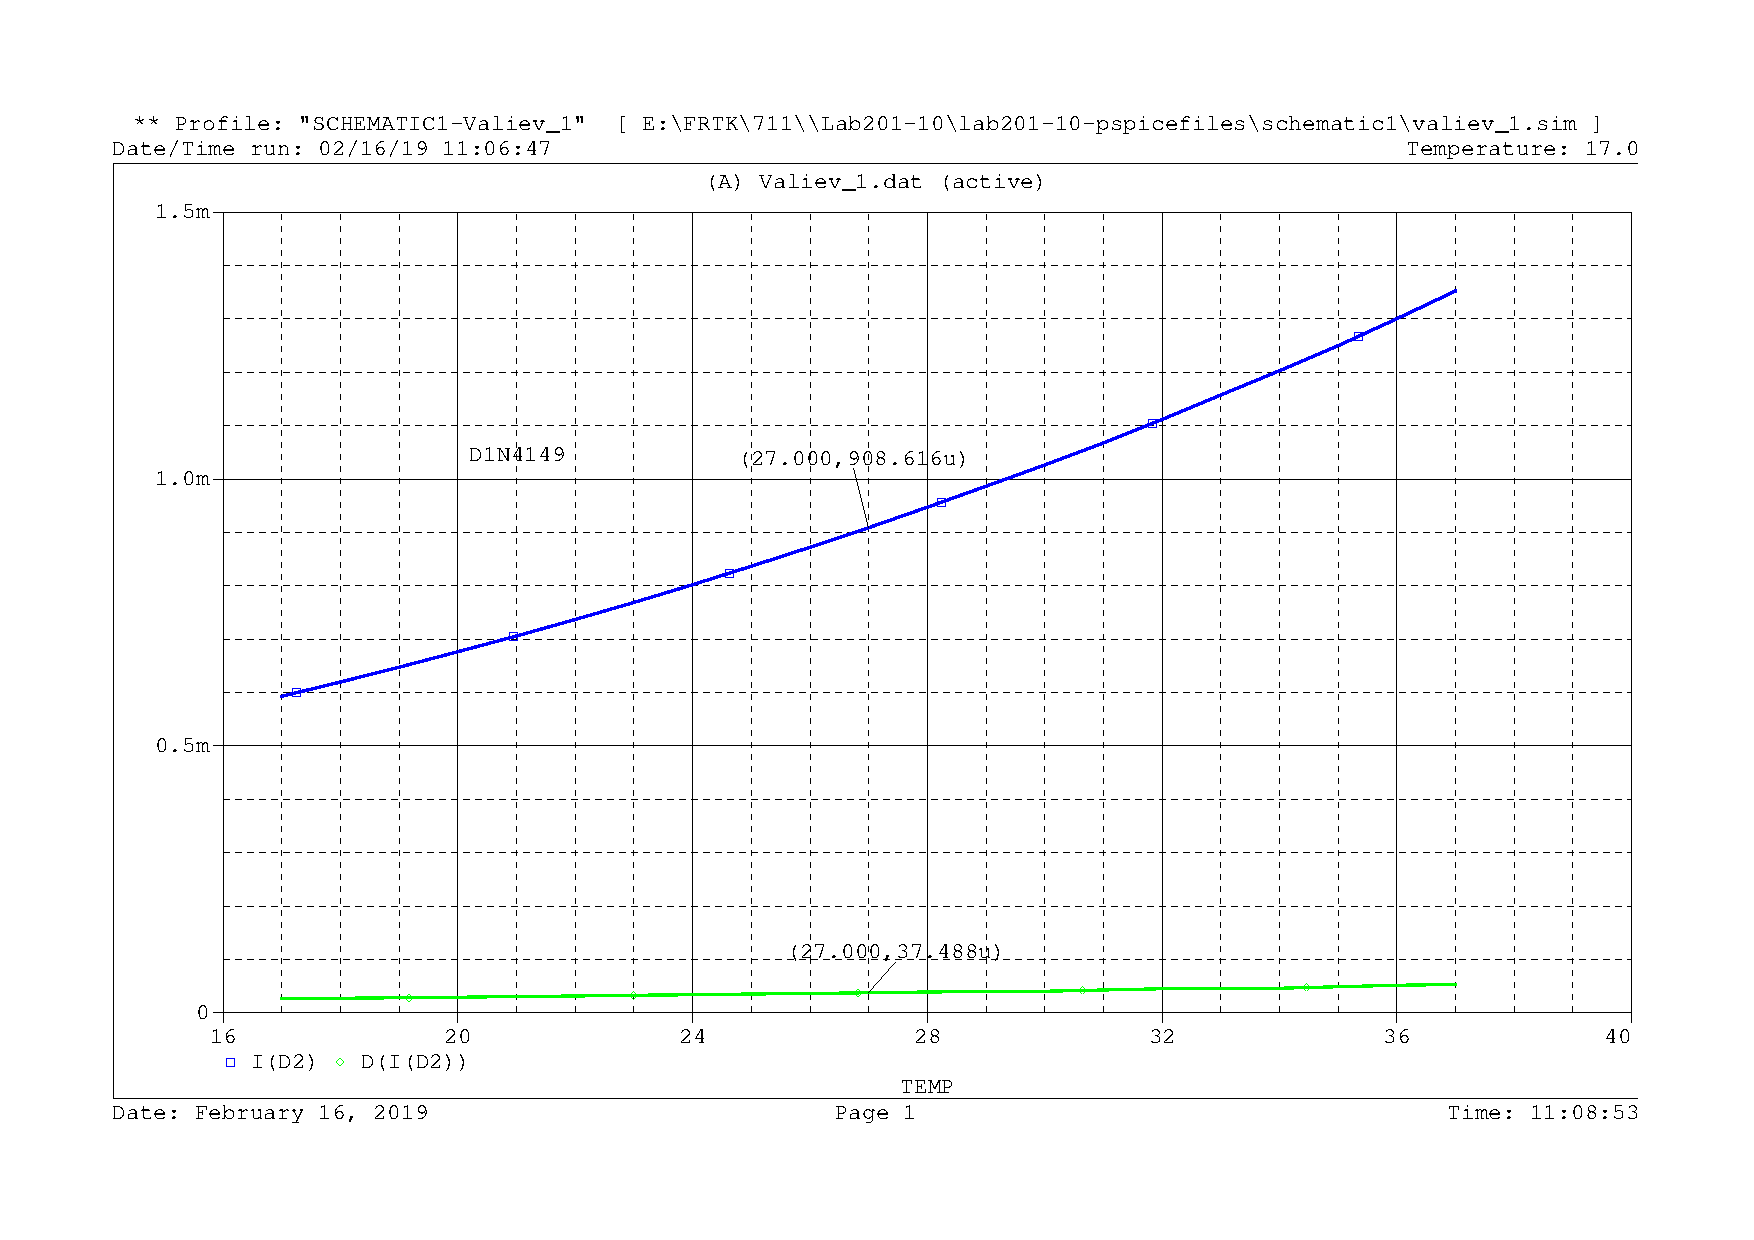
\includegraphics[width = 0.9 \textwidth]{16}
	\caption{R1 = R2 = 100}
\end{figure}

\newpage





\textbf{{\normalsize 5:}}
Составим схему (рис. \ref{scheme_3}) моделирования процессов МОП транзисторов. Получим временные диаграммы токов стоков ID(M1), ID(M2) при трех значениях R1, R2: 1, 100, 1000.
\begin{figure}[H]
	\centering
	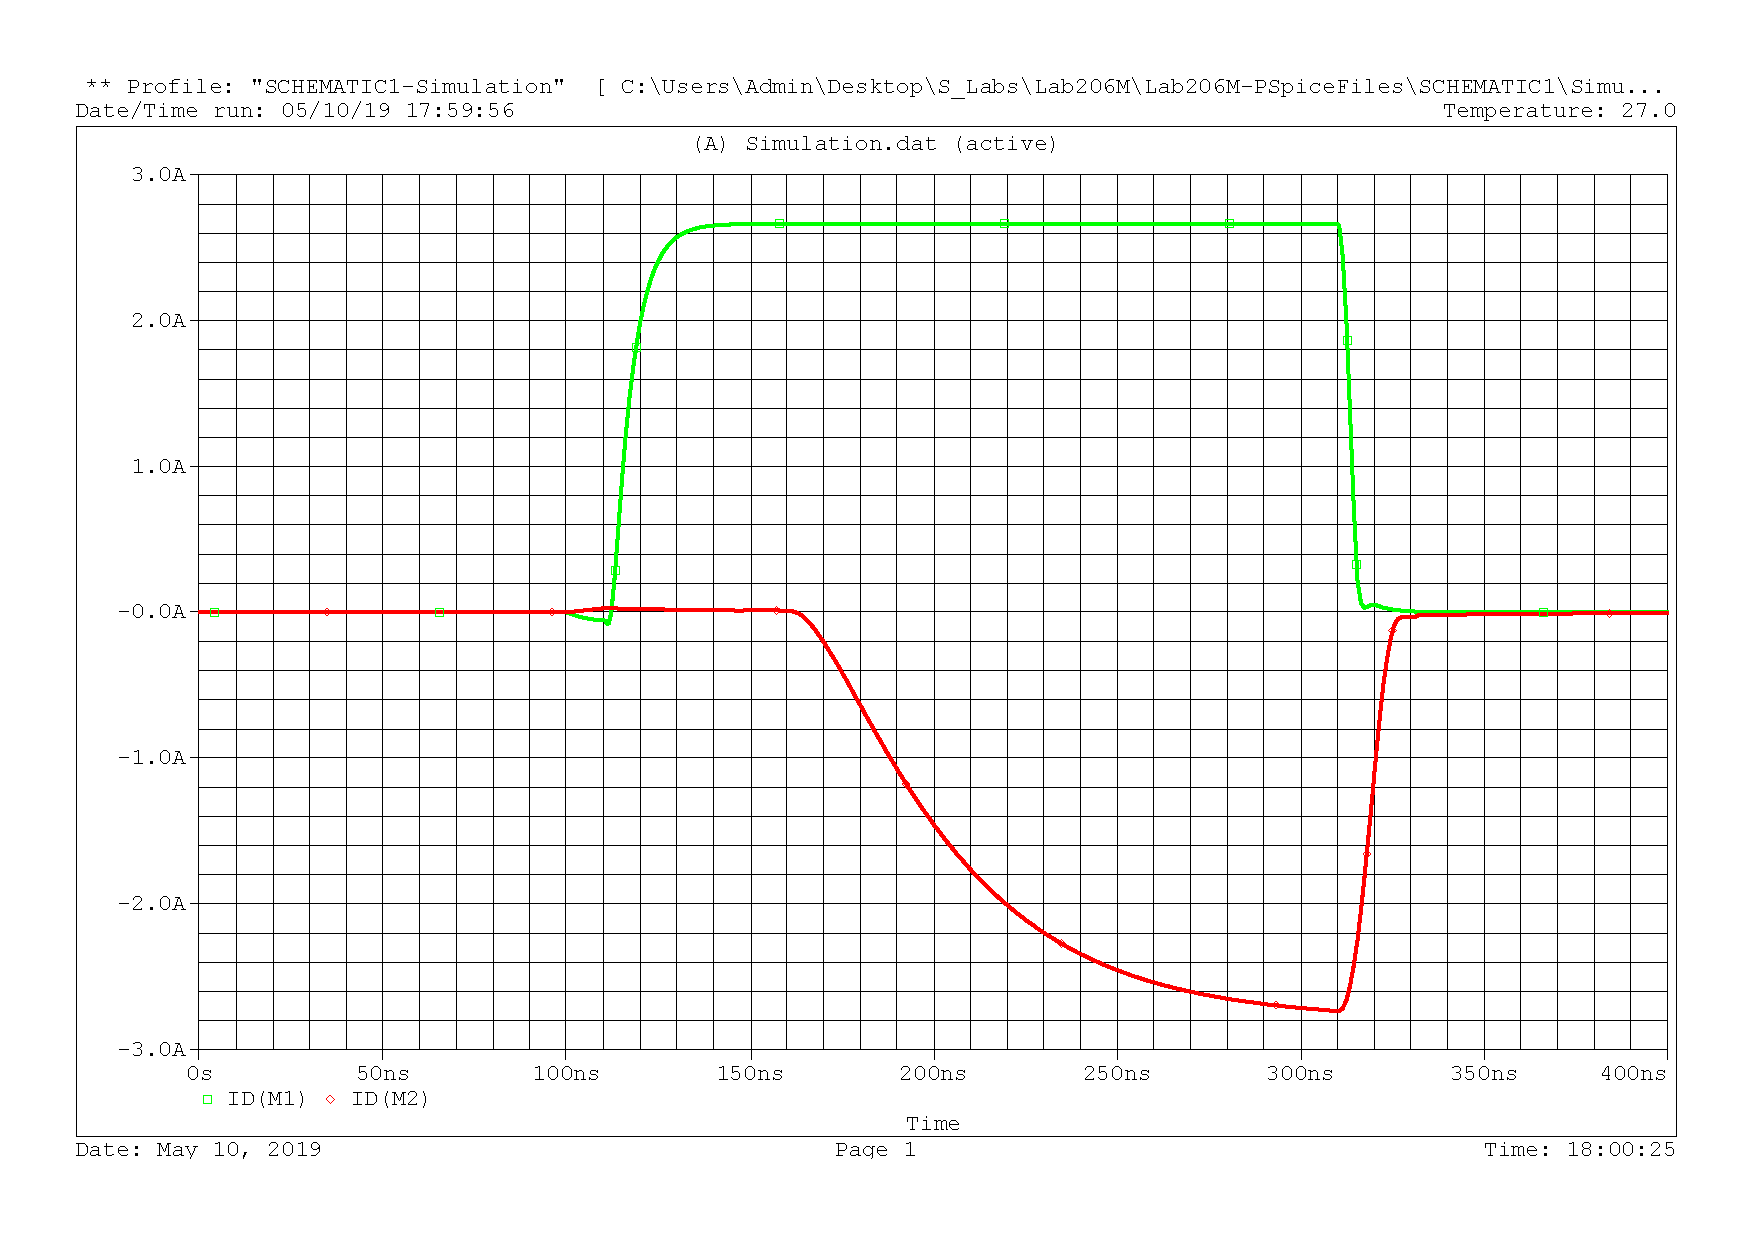
\includegraphics[width = 0.9 \textwidth]{17}
	\caption{R1 = R2 = 1}
\end{figure}

\begin{figure}[H]
	\centering
	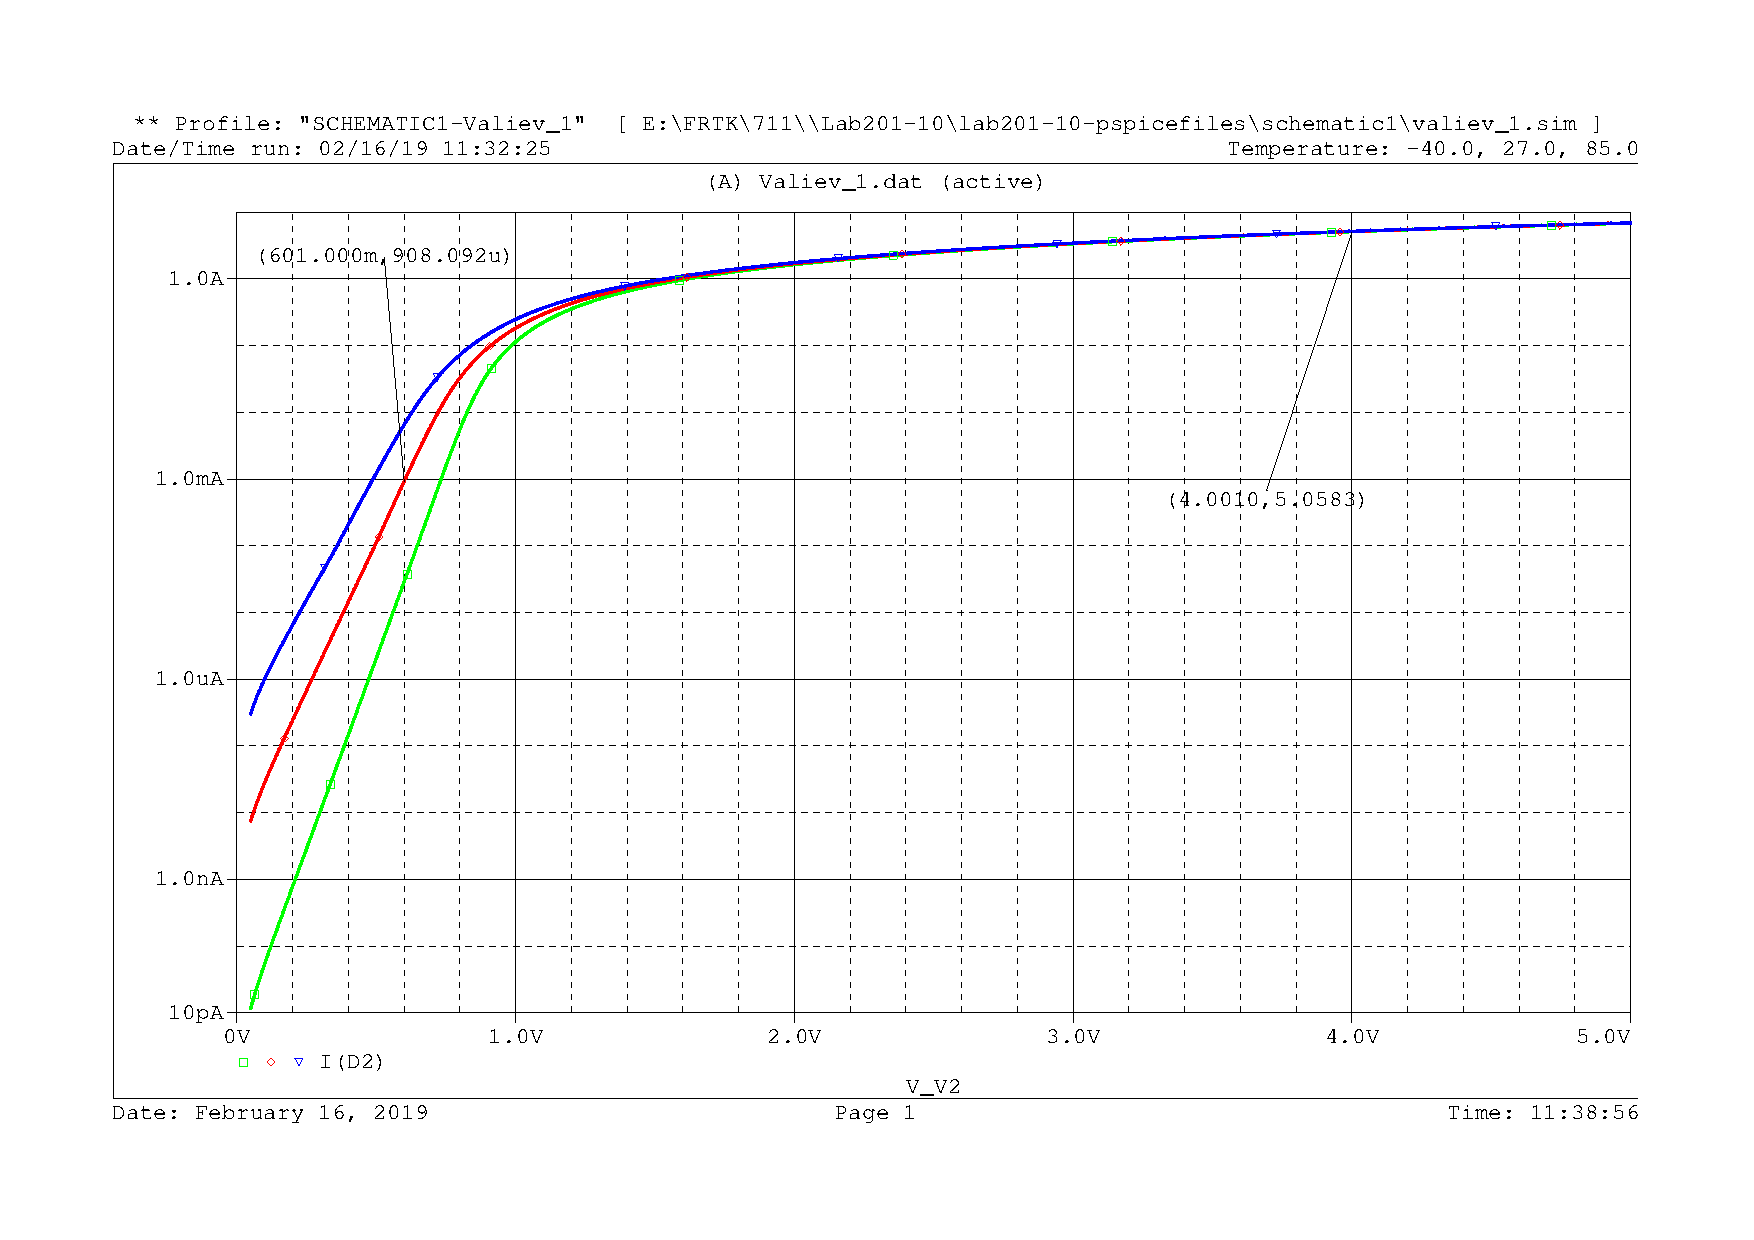
\includegraphics[width = 0.9 \textwidth]{18}
	\caption{R1 = R2 = 100}
\end{figure}

\begin{figure}[H]
	\centering
	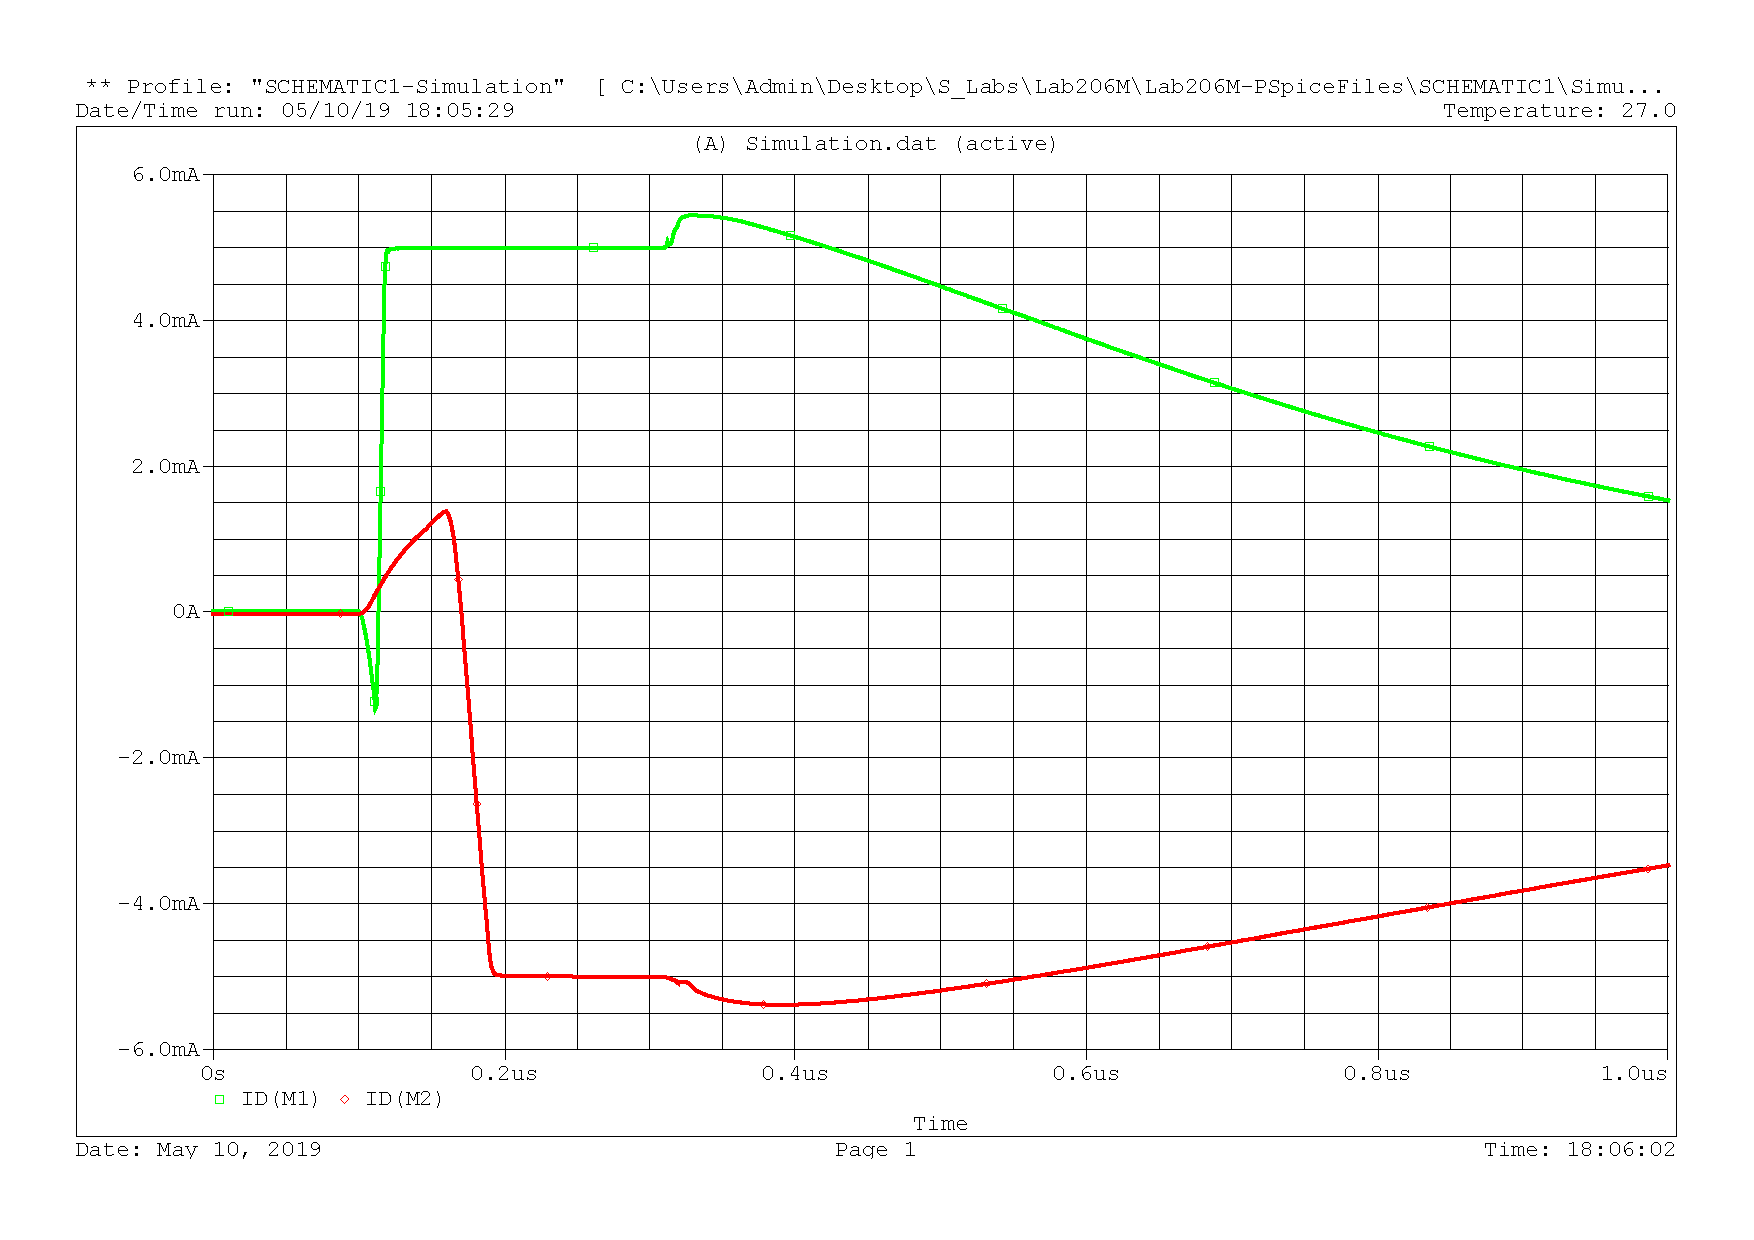
\includegraphics[width = 0.9 \textwidth]{19}
	\caption{R1 = R2 = 1000}
\end{figure}

\end{document}